\documentclass[11pt]{article}

\usepackage{makeidx}

\usepackage{latexsym}

\usepackage{color}

\usepackage{wrapfig}

\usepackage{here}

\usepackage{graphicx}

\usepackage[centertags]{amsmath}

\usepackage{amsfonts}

\usepackage{amssymb}

\usepackage{amsthm}

\usepackage{subfigure}

\usepackage{here}

\usepackage{ulsy}

\usepackage{hyperref}


\addtolength{\topmargin}{-2.5cm}

\addtolength{\textheight}{4cm}

\addtolength{\oddsidemargin}{-2cm} \addtolength{\textwidth}{3.5cm}

\addtolength{\evensidemargin}{-2cm}



\begin{document}

\renewcommand\floatpagefraction{.9}

\renewcommand\topfraction{.9}

\renewcommand\bottomfraction{.9}

\renewcommand\textfraction{.1}

\setcounter{totalnumber}{50} \setcounter{topnumber}{50}

\setcounter{bottomnumber}{50} \floatsep 20 pt \intextsep 5 pt

\abovecaptionskip 0 pt

\belowcaptionskip 0 pt



\newcommand{\beq}{\begin{equation}}

\newcommand{\eeq}{\end{equation}}

\newcommand{\ba}{\begin{array}}

\newcommand{\ea}{\end{array}}

\newcommand{\bea}{\begin{eqnarray}}

\newcommand{\eea}{\end{eqnarray}}

\newcommand{\bes}{\begin{eqnarray*}}

\newcommand{\ees}{\end{eqnarray*}}

\newcommand{\vs}{\vspace*{0.5cm}}

\newcommand{\svs}{\vspace*{0.25cm}}



\newcommand{\abs}[1]{\mid \! #1\! \mid}

\renewcommand{\b}[1]{\mbox{{\bf #1}}}

\renewcommand{\vec}[1]{\protect\overrightarrow{ #1}}

\newcommand{\mat}[1]{\mbox{\boldmath $#1$}}



\long\def\bform#1\eform{\begin{equation}

   \begin{minipage}{\eqbreite}\vskip .1cm

   \let\\ = \thcr

   \halign{$\displaystyle{##}$ \hfil

  && $\displaystyle{##}$\hfil\cr#1\cr}

   \vskip .3cm \end{minipage}

\end{equation}}

\def\thcr{\cr\noalign{\vskip.3cm}}

\newlength{\eqbreite}\setlength{\eqbreite}{\textwidth}

\addtolength{\eqbreite}{-1.5cm}



\long\def\bnn#1\enn{$$\begin{minipage}{\eqbreite}

\vskip .1cm \let\\ = \thcr \halign{$\displaystyle{##}$

\hfil && $\displaystyle{##}$\hfil \cr#1 \cr}

\vskip.3cm \end{minipage}$$}



\parindent 0 in

\parskip .25 cm



\input epsf



%%%%%%%%%%%%%%%%%%%%%%%%%%%%%%%%%%%%%%%%%%%%%%%%%%%%%%%%%%%

% Actual text starts below:

%%%%%%%%%%%%%%%%%%%%%%%%%%%%%%%%%%%%%%%%%%%%%%%%%%%%%%%%%%%



\thispagestyle{empty}

\svs

\begin{center}

\begin{huge}
  \textrm{\textbf{Maths	{\textcolor{red}{\Huge 4}}Biology}}\\
\end{huge} 
\vspace*{1cm}
\begin{Large}
  {\bf Alberto Pascual-Garc{\'i}a} \\
\end{Large}

\end{center} \vs



\normalsize
This project contains supporting notes and scripts for the course "Maths for Biology"
of the Master for Computational Methods in Ecology and Evolution at 
Imperial College London. It is a \href{}{fork} of the the 
\href{https://github.com/vjirsa/bootcamp}{project} "Mathematics Boot Camp" proposed
by \href{http://ins.univ-amu.fr/research-teams/team-member/v.jirsa/}{Viktor Jirsa}
for graduate courses at the Center for Complex Systems \& Brain Sciences at Florida
Atlantic University. Similar in spirit, by no means it is intended to compete with the
traditional introductory courses in mathematics taught at universities. Rather it should
be viewed as a synopsis of the mathematical tools most probably encountered in scientific
applications. With respect to Jistra's notes, the present project expands
some of the topics, and it further includes First-Order Differential Equations, of oustanding importance
in Ecology. On the other hand, Fourier analysis is not considered in the course, although it is kept in the repository for completeness.

\vs \svs



\begin{figure}[!h]

    \centerline{\epsfxsize=10cm  \epsfbox{FRONT_COVER.ps}}

\end{figure} \vs \svs



\begin{center} \Large

\textrm{Z{\"u}rich, December 2018 \\
     Institute of Integrative Biology \\
     ETH}
\end{center}  \normalsize



\newpage

\vspace{5cm}
\begin{center} \Large
  \textrm{{\bf LICENSE -- DOCUMENT}\\
    \vs
    Copyright (c) 2018 Viktor K. Jirsa and Alberto Pascual-Garc{\'i}a}
\end{center} \normalsize \vs \svs



This work is licensed under the Creative Commons Attribution-NonCommercial-ShareAlike 4.0 International License. 
To view a copy of this license, visit \href{http://creativecommons.org/licenses/by-nc-sa/4.0/}{this page} or send a letter 
to Creative Commons, PO Box 1866, Mountain View, CA 94042, USA.

\vspace{3cm}

%\begin{figure}
%
%    \centerline{\epsfxsize=11cm \includegraphics{CC-license.eps}}
%
%\end{figure} \vs \svs


\vspace{5cm}
\begin{center} \Large
  \textrm{{\bf LICENSE -- \href{https://www.flickr.com/photos/anroir/323864105/}{PICTURE COVER}}\\
    \vs
    Copyright (c) 2016 anroir \href{https://www.flickr.com/people/anroir/}{(https://www.flickr.com/people/anroir/)}}
\end{center} \normalsize \vs \svs


The picture in the cover of the document is licensed under a Creative Commons Attribution-NonCommercial 2.0 International License. 
To view a copy of this license, visit \href{https://creativecommons.org/licenses/by-nc/2.0/}{this page} or send a letter 
to Creative Commons, PO Box 1866, Mountain View, CA 94042, USA.


\newpage

\tableofcontents

\listoffigures



\newpage

\pagestyle{plain}



%\setcounter{page}{1}

\section{Function Theory}
\subsection{Foundations}

{\bf Definition:} Consider two sets of elements $A$ and $B$. A {\em function} $f$ is a rule which unambiguously
assigns $y \in B$ to each $x \in A$. We call the set $A$ the {\em domain} of the function and the set $B$ its
{\em codomain}.

{\bf Note:} "$x \in A$" means that "$x$ is an element of $A$".\vs

\begin{figure}[!h]
    \centerline{\epsfxsize=10cm  \epsfbox{matlab/fig1.eps}} \vs
    \caption{Illustration of a function} \label{fig1}
\end{figure} \vs

{\bf Notation:}
\bnn \begin{array}{ccc}
    f: & A \rightarrow B & \\ \svs
    f: & A \rightarrow B & \;\; x\in A, \; y\in B \\ \svs
    & y = f(x) & \;\; x\in A, \; y\in B \\ \svs
    & y = y(x) & \;\; x\in A, \; y\in B
\end{array} \enn \vs

{\bf Examples:}

\vs \begin{figure}[!h]
   \centerline{\epsfxsize=10cm \epsfbox{matlab/fig2.eps}} \vs
   \caption{Assigning an element $\{21\} \in B$ to $\{1\} \in A$} \label{fig2}
\end{figure} \vs

\newpage

Most commonly, functions are defined by equations: \qquad a) $ y = f(x) = 2x + 1$, \qquad b) $y=f(x)=x^2$  \svs

{Graphical representation:} \svs
\begin{figure}[!h]
    \centering
    \subfigure[Function $y = 2x + 1$]{\epsfxsize=7cm \epsfbox{matlab/fig3a.eps}}
    \hspace*{0.5cm}
    \subfigure[Function $y = x^2$]{\epsfxsize=7cm \epsfbox{matlab/fig3b.eps}} \svs
    \caption{A linear and a quadratic function} \label{fig3}
\end{figure} \vs

{\bf Types:} Some important types of functions are:
\begin{enumerate}
\item Injective functions: Those functions that preserve distinctiveness, i.e. they never map distinct elements of its domain to the same elements of its codomain.
\item Surjective functions: Every element $y$ of the codomain has a correspondent element $x$ of the domain that is mapping it.
\item Bijective functions: Those functions that are both injective and surjective.
\end{enumerate}

\subsection{Domain, parity and periodicity of functions}

{\bf Domain of a function} is the set of input values in which the function can be defined. Therefore, given
a map between two sets, to define a function we should determine a valid domain identifying possible {\em pathological} input values.

{\bf Example:} 
The map $f(x) = 1/x$ has a pathological value at $x=0$ meaning that the map diverges to infinity. In order
for this map to be a function, we should {\em restrict the domain} and define the function as:

\bnn 
  f(x)=\begin{cases}
    1/x, & \text{if $x\neq0$}.\\
    0, & \text{if $x=0$}.
  \end{cases}
\enn

{\bf Parity of a function.} Let $f(x)$ be a real-valued function, then:
\begin{enumerate}
 \item $f$ is {\em even} if the following equation holds for all $x$ in the domain of $f$:
 		\bnn f(x) = f(-x) \quad \rightarrow \quad f(x)-f(-x)=0 \enn
 \item $f$ is {\em odd} if
 	    \bnn -f(x) = f(-x) \quad  \rightarrow \quad f(x)+f(-x)=0.\enn
\end{enumerate}

{\bf Note:} These properties will be very useful to guess some properties of derivatives and integrals of functions.

{\bf Periodicity of a function.} We say that a function $f(x)$ is periodic if for all $x$ in the domain of $f$ there is a value $\lambda \in \mathbb{R}$ such that for a every $n \in \mathbb{N}$ it holds that $f(x) = f(x+n\lambda)$, where $\lambda$ is the {\em period} of the function.

\subsection{Inverse Functions}

$f^{-1}$ denotes the inverse of the function $f$. \vs

\begin{figure}[!h]
   \centerline{\epsfxsize=11cm  \epsfbox{matlab/fig4.eps}} \svs
    \caption{Inverse function} \label{fig4}
\end{figure} \vs

{\bf Notation:}
\bnn f^{-1}: \; B \rightarrow A \enn \svs
\bnn x = f^{-1}\,(y) \qquad \mbox{where} \qquad y = f(x) \enn \svs

Graphically the inverse can be constructed as the mirror image of the function at the
first bisector. This method always works, but caution is asked for, because the inverse 
may not be unique and require more detailed discussion.

{\bf Example:}
\bnn y = f(x) = 2x + 1  \qquad  x = f^{-1}\,(y) = \frac{1}{2} \, (y-1) \enn

{\bf Note:} There is not always an inverse function!  \vs

\begin{figure}[!h]
   \centerline{\epsfxsize=11cm \epsfbox{matlab/fig5.eps}} \svs
    \caption{The inverse $f^{-1}$ is not unique, thus not a function.} \label{fig5}
\end{figure} \vs


{\bf Example:}
\bnn y = f(x) = x^2 \enn
\bnn x = \sqrt{y} \qquad \mbox{or} \qquad x = -\sqrt{y} \enn  \vs

\begin{figure}[!h]
    \centering
    \subfigure[$\; f(x)=2\,x+1 \; \rightarrow \; f^{-1}(x)=\frac{1}{2}(x-1)$]{\epsfxsize=7cm \epsfysize=7cm
        \epsfbox{matlab/fig6a.eps}}
    \hspace*{0.5cm}
    \subfigure[$\; f(x)=x^2 \; \rightarrow \; f^{-1}(x)=\pm\sqrt{x}$]{\epsfxsize=7cm \epsfysize=7cm
         \epsfbox{matlab/fig6b.eps}} \svs
    \caption{Graphical construction of the inverse function} \label{fig6}
\end{figure}

\newpage
\subsection{Implicit Functions}
A function is not given explicitly as in $y = f(x)$, but
implicitly by $F(x,y) = 0$. Note that an implicit equation may not necessarily fulfill
the conditions of a function when written explicitly, unless some additional conditions
are imposed.

{\bf Example:} Unit circle: $\quad F(x,y)=x^2+y^2-1=0$. In the plot, we observe that
each $x$ point corresponds to two $y$ points and hence it is not a function. \svs

\begin{figure}[!h]
    \centerline{\epsfxsize=7cm \epsfysize=7cm \epsfbox{matlab/fig7.eps}} \svs
    \caption{Unit circle} \label{fig7}
\end{figure} \svs

The implicit representation of the unit circle needs additional conditions to become
unique and thus a function: a local neighborhood has to be defined, e.g. $y=\sqrt{1-x^2}$
for \mbox{$x\in (-1;1)$},  \mbox{$y >0$} and $y=-\sqrt{1-x^2}$ for $x\in (-1;1), \, y<0$.

{\bf Note:} The implicit representation is particularly important for algebraic equations
of the form:

\bnn
a_n(x)y^n + a_{n-1}y^{n-1}+...+a_0(x)=0
\enn

since those of order $n>5$ may not have an explicit representation.

\subsection{Polynomials}
Polynomials are defined as a class of functions of the form
\bnn y = a_0 + a_1 \, x + a_2 \, x^2 + \dots + a_N \, x^N = \sum_{n=0}^N a_n \, x^n \enn
where the function $y$ is said to be a polynomial of order $N$.  \svs

{\bf Example:}
\bnn y = \underbrace{2}_{a_2} x^2 + \underbrace{8}_{a_1} x + \underbrace{4}_{a_0} \enn

{\bf Goal:} To achieve a qualitative understanding of a given function without computing each value.

{\bf Approach:}
\bnn y = \sum_{n=0}^N a_n \, x^n  \qquad \mbox{where we assume} \;\; a_N>0 \enn

\begin{description}
\item[{\bf Step 1:}] If $N$ is even, then $x \rightarrow \pm\infty : y \rightarrow \pm \infty \, ; \quad$
if $N$ is odd, then $x \rightarrow \pm \infty : y \rightarrow \mp \infty$. Note: If $a_N<0$,
the behavior is the opposite.
\item[{\bf Step 2: (Fundamental theorem of algebra)}] A polynomial of order $N$ has $N$ roots which are the solutions of $f(x)=0$.

Set $y=0: f(x) = x^N + a_{N-1}\, x^{N-1} + \dots + a_1 \,x + a_0 = 0 $
\bnn \begin{array}{ccl} \svs
y = 17x + 4 \quad & y=0: x=-\frac{4}{17} & \quad \rightarrow  \quad \mbox{1 root} \\
y = 2x^2 + 8x + 4 \quad & y=0: x=\frac{1}{4}(-8 \pm \sqrt{8^2-4\cdot2\cdot4})=\frac{1}{4}(-8 \pm
\sqrt{32)}=-2 \pm \sqrt{2} & \quad \rightarrow \quad  \mbox{2 roots}
\end{array} \enn
\begin{center}
    $\Rightarrow$ the roots are the locations where $f(x)$ crosses the $x$-axis.
\end{center}
\end{description}

{\bf Note:} Analytic formulas to find the roots of polynomials are known until 4th degree.

{\bf Examples:} Construct graph of $y=f(x)$ \vs
\begin{figure}[!h]
\centering \subfigure[Step 1: $y=x^2+3x+2$] {\epsfxsize=7cm \epsfbox{matlab/fig8a.eps}}
\hspace*{0.5cm}
\subfigure[Step 2:  $y=x^2+3x+2=0$] {\epsfxsize=7cm \epsfbox{matlab/fig8b.eps}} \svs 
\caption{Graphical construction (the roots are $x=-1$ and $x=-2$)} \label{fig8}
\end{figure}

\vs\vs\begin{figure}[!h]
\centering \subfigure[Step 1: $y=x^3+2x^2-3x$] {\epsfxsize=7cm \epsfbox{matlab/fig9a.eps}}
\hspace*{0.5cm}%
\subfigure[Step 2: $y=x^3+2x^2-3x=0$] {\epsfxsize=7cm \epsfbox{matlab/fig9b.eps}} \svs 
\caption{Graphical construction (the roots are $x=-3, x=0$ and $x=1$)} \label{fig9}
\end{figure}

\begin{figure}[!h]
\centering \subfigure[Step 1: $y=x^4+2x^3-3x^2$] {\epsfxsize=7cm \epsfbox{matlab/fig10a.eps}}
\hspace*{0.5cm}%
\subfigure[Step 2: $y=x^4+2x^3-3x^2=0$] {\epsfxsize=7cm \epsfbox{matlab/fig10b.eps}} \svs 
\caption{Graphical construction (the roots are $x=-3, x=0$ and $x=1$)} \label{fig9}
\end{figure} 

\newpage

{\bf Horizontal translation} is a horizontal shift of a function by $x_0$
\bnn y=f(x) \; \rightarrow \; y =f(x-x_0) \enn

{\bf Example:} $\qquad y = x^2$  \; shift by $\; x_0=2$: \; $ y = (x-2)^2 = x^2 - 4x +4$  \vs

\vs {\bf Vertical translation} is a vertical shift of a function by $y_0$
\bnn y=f(x) \; \rightarrow \; y =f(x)+y_0 \enn

{\bf Example:} $\qquad y=x^2$ \; shift by $\; y_0=2$: \;  $ y=x^2+2 $ \vs

\vs\begin{figure}[!h]
\centering \subfigure[Horizontal shift by $x_0=2: y=(x-2)^2$]{\epsfxsize=7cm \epsfbox{matlab/fig11a.eps}} 
\hspace*{0.5cm}
\subfigure[Vertical shift by $y_0=2: y = x^2+2$] {\epsfxsize=7cm \epsfbox{matlab/fig11b.eps}} \svs 
\caption{Vertical and horizontal shift of $y=x^2$} \label{fig11}
\end{figure}

\subsection{Rational functions}

Given two polynomial functions $D(x)$ and $d(x)$ a rational function has the form:
\bnn f(x)=\frac{D(x)}{d(x)} \enn

Working with these functions can be cumbersome if the polynomials are complicated. It is
useful to learn how to factorize the polynomials, because it will allow us to find equivalent
(simplified) functions. 

{\bf 1. Binomial expressions.} Second order polynomials can be factorized in the product of two first order polynomials, i.e. $ax^2+bx+c = (x+u)(x+v)$. Some immediate factorizations are:

\bnn
 	a^2x^2+b^2+2abx=(ax+b)(ax+b)\\
 	a^2x^2+b^2-2abx=(ax-b)(ax-b)\\
    a^2x^2-b^2=(ax+b)(ax-b)
\enn 

Nevertheless, other expressions are not so easy. In general, we know that we are looking
for something like $(x+u)(x+v)$ and hence, if we have for instance

\bnn x^2+bx+c = (x+u)(x+v)= x^2 + (u+v)x + uv, \enn

we can see that $u+v=b$ and $uv=c$, which are two equations with two unknowns that we can solve. A little
bit more general expression would be:

\bnn ax^2+bx+c = (ax+u)(x+v)= ax^2 + (u+av)x + uv, \enn

leads to $u+av=b$ and $uv=c$. 

{\bf Example:}

\bnn
\frac{x^4+8x^2+7}{3x^5-3x} = \frac{(x^2+7)(x^2+1)}{3x(x^2+1)(x^2-1)} = \frac{x^2+7}{3x(x^2-1)}
\enn

%If we substitute $u=c/v$ in the first equation
%we get $c+av^2=bv \quad\rightarrow \quad v=\frac{-b\pm\sqrt{b^2-4ac}}{2a}$ and only one of the
%solutions will be compatible with the second equation $u=c/v$. However, the factorization
%of $c$ in prime numbers typically brings an immediate answer.

{\bf 2. Degree of $D(x)$ is larger than $d(x)$. } In this situation we can simply divide the numerator
by the denominator! Calling $q(x)$ to the quotient and $r(x)$ to the remainder of the division, we get:

\bnn
	\frac{D(x)}{d(x)}=q(x)+\frac{r(x)}{d(x)}.
\enn

{\bf Example:}

\bnn
	\frac{3x^3-2x^2+4x-3}{x^2+3x+3}=(3x-11)+\frac{28x+30}{x^2+3x+3},
\enn

{\bf 3. Degree of $D(x)$ is smaller than $d(x)$. } To solve this case we proceed in three steps that we illustrate with one example:

{\em Step 1 --} Factorize the denominator.
\bnn
	\frac{x}{x^2-3x+2}=\frac{x}{(x-1)(x-2)}
\enn
{\em Step 2 --} Rewrite the function as a sum of rational functions whose numerators are polynomials of degree zero, sum up the functions and group the terms by their degree on $x$.
\bnn
	\frac{x}{(x-1)(x-2)}=\frac{A}{(x-1)}+\frac{B}{(x-2)}=\\
	=\frac{A(x-2)+B(x-1)}{(x-1)(x-2)}=\frac{(A+B)x-(2A+B)}{(x-1)(x-2)}
\enn
{\em Step 3 --} Identify the terms in the numerator of the last expression with those of the original function, and find the coefficients $A$, $B$, etc.
\bnn
	(A+B)x-(2A+B) = x.
\enn

Since the coefficient of $x$ in the numerator of the original function is 1 we get $A+B=1$ and, since the independent term is zero, we get $2A+B=0$. Considering both equations for the variables $A$ and $B$ we conclude that $A=-1$ and $B=2$, and the final factorization is:
\bnn
	\frac{x}{(x-1)(x-2)}=\frac{-1}{(x-1)}+\frac{2}{(x-2)}
\enn

{\bf Example:} It may happen that the multiplicity of any of the factors in the denominator is larger than one, in which case the decomposition at Step 2 becomes:

\bnn
	\frac{x}{(x-1)^3}=\frac{A}{(x-1)}+\frac{B}{(x-1)^2}+\frac{C}{(x-1)^3}
\enn

and we proceed similarly

\bnn
	\frac{x}{(x-1)^3}=\frac{A(x-1)^2+B(x-1)+C}{(x-1)^3}=\frac{Ax^2+(B-2A)x+(A+C-B)}{(x-1)^3}
\enn

finding that $A=0$, $B=1$ and $C=1$.

\subsection{Trigonometric Functions}
Trigonometric functions are a class of periodic functions such as
\bnn y = f(x) = A \sin(kx + \phi) \quad \mbox{and} \quad
     y = f(x) = A \cos(kx + \phi) \enn

The constant parameters are the amplitude
$A$, the frequency $k$ and the phase (angle) $\phi$. The period is
defined as $\lambda=2\pi/k$ and the trigonometric functions fulfill
the relation $f(x+\lambda)=f(x)$.
\small  \vspace*{-5mm} \begin{center} \begin{tabular}{|c|c|c|c|c|c|c|c|c|} \hline
\multicolumn{9}{|c|} {Special values of trigonometric functions (midnight stuff)\rule{0pt}{4mm}} \\
\hline \hline
$x$ & $\;0\;$ & $\pi/6=30^{\circ}$ & $\pi/4=45^{\circ}$ & $\pi/3=60^{\circ}$ & $\;\pi/2=90^{\circ}\;$ & $\;\pi=180^{\circ}\;$
 & $\;3\pi/2=270^{\circ}\;$ & $\;2\pi=360^{\circ}\; $  \rule{0pt}{4mm} \\
\hline
$\;\sin x\;$ & $0$ & $1/2$ & $\sqrt{2}/2$ & $\sqrt{3}/2$ & $1$ & $0$ & $-1$ & $0$  \rule{0pt}{4mm} \\
\hline
$\cos  x$    & $1$ & $\sqrt{3}/2$ & $\sqrt{2}/2$ & $1/2$ & $0$ & $-1$ & $0$ & $1$ \rule{0pt}{4mm} \\
\hline
\end{tabular} \end{center} \normalsize

Horizontal translation (shift) by means of $\phi$:
\bnn
\sin(x+\frac{\pi}{2})=\cos{x} \qquad \cos(x+\frac{\pi}{2})=-\sin{x} \qquad
\sin(x-\frac{\pi}{2})=-\cos{x} \qquad \cos(x-\frac{\pi}{2})=\sin{x}
\enn

Useful relations between $\cos{x}$ and $\sin{x}$:
\bnn \cos^2{x}+\sin^2{x}=1 \enn
\bnn \sin(x\pm y)=\sin{x}\cos{y} \pm \cos{x}\sin{y} \qquad
\cos(x\pm y) = \cos{x}\cos{y} \mp \sin{x}\sin{y} \enn
\bnn \sin{2x} = 2\sin{x}\cos{x} \qquad
\cos{2x} = \cos^2{x} - \sin^2{x} \enn

Other trigonometric functions:
\bnn \tan{x} = \frac{\sin{x}}{\cos{x}} \qquad\qquad \cot{x} = \frac{\cos{x}}{\sin{x}} \enn

\begin{figure}[!h]
\centering 
\subfigure[The functions  $y\!=\!\sin{x}$ and \mbox{$y\!=\!\cos{x}$}] {\epsfxsize=7cm \epsfbox{matlab/fig12a.eps}}
\hspace*{0.5cm}
\subfigure[The functions $y\!=\!\tan{x}$ and $y\!=\!\cot{x}$. Note that these are $\pi$-periodic]
           {\epsfxsize=7cm \epsfbox{matlab/fig12b.eps}} \svs
\caption{The most common trigonometric functions} \label{fig12}
\end{figure}


\subsection{Exponential Functions}

Exponential functions are functions most commonly used in the form
\bnn y = A e^{kx} = A \exp{k x} \enn
with the constant parameters: $A$ amplitude, $k$ growth rate if $k>0$ and the damping or fall 
off, if $k<0$, and $e$ Euler number: 2.718....

Note that $e^0=1\;$ and $\;e^{-x}=\frac{1}{e^x}$. \svs

\begin{figure}[!h]
    \centerline{\epsfxsize=10cm \epsfbox{matlab/fig13.eps}}
    \caption{Exponential functions} \label{fig13}
\end{figure} \vs


\subsection{Hyperbolic Functions}

Hyperbolic functions are of the form
\bnn y = f(x) = \cosh{x} = \frac{1}{2}(e^x + e^{-x}) \qquad\mbox{hyperbolic cosine} \enn
and
\bnn y = f(x) = \sinh{x} = \frac{1}{2}(e^x - e^{-x}) \qquad\mbox{hyperbolic sine} \enn

They have similar properties as the trigonometric functions such as a representation by
exponentials (as we shall see later), and their derivatives convert into each other. 
But the hyperbolic functions are {\em not} periodic. \vs

Other hyperbolic functions:
\bnn
y=\tanh{x}=\frac{\sinh{x}}{\cosh{x}}=\frac{e^{x}-e^{-x}}{e^{x}+e^{-x}} \qquad
y=\coth{x}=\frac{\cosh{x}}{\sinh{x}}=\frac{e^{x}+e^{-x}}{e^{x}-e^{-x}}
\enn

\begin{figure}[!h]
    \centering
    \subfigure[$y=\sinh{x}\;$ and $\;y=x+\frac{1}{3!}\,x^3$]{\epsfxsize=7cm \epsfbox{matlab/fig14b.eps}}
    \hspace*{0.5cm}
    \subfigure[$y=\cosh{x}\;$ and $\;y=1+\frac{1}{2!}\,x^2$]{\epsfxsize=7cm \epsfbox{matlab/fig14a.eps}} \svs
    \caption{Hyperbolic functions} \label{fig14}
\end{figure} \vs



\subsection{Basic Inverse Functions}
\subsubsection{Logarithms}
The logarithms are the inverse of the exponential functions:
\bnn y=a^x \quad \leftrightarrow \quad x = \log_a y  \qquad\mbox{where} \quad 0<y<\infty \enn

{\bf Special cases:}
\begin{eqnarray*}
\begin{array}{lcccccc}
a=e: \qquad & y & = & \log_e x & = & \ln x & \qquad\mbox{natural logarithm}\\
a=10: \qquad & y & = & \log_{10} x & = & \mbox{lg} x & \qquad\mbox{decimal logarithm}\\
a=2: \qquad  & y & = & \log_2 x & = & \mbox{ld} x & \qquad\mbox{dual logarithm}
\end{array}
\end{eqnarray*}

\begin{figure}[!h]
    \centerline{\epsfxsize=10cm  \epsfbox{matlab/fig15.eps}} \svs
   \caption{The logarithmic functions $y=\ln(x)$, $y=\mbox{lg}(x)$, $y=\mbox{ld}(x)$, and $y=-\ln(x)$.} \label{fig15}
\end{figure} \vs

{\bf Remark:} The most commonly used logarithm is $\ln x$, but there are certain applications for other 
logarithms as well. For instance, the decimal logarithm can be used to find the number of digits in 
a decimal number 
($\mbox{lg} 4821=3.683 \rightarrow$  taking the whole number in front of the decimal point and 
adding 1 gives the number of digits, 4). Similarly, the dual logarithm can be used to find the number
of bits or binary digits that are necessary to represent a number $n$ in binary format, i.e. as 
zeros and ones.  

{\bf Rules and tricks for dealing with logarithms:}
\bnn \log_a x^n = n \log_a x \enn
\bnn \log_a x_1 \, x_2 = \log_a x_1 + \log_a x_2  \qquad  \log_a \frac{x_1}{x_2} = \log_a x_1 - \log_a x_2  \enn
\bnn \log_a x = \frac{\log_b x}{\log_b a} \enn

{\bf Note:} The last expression tells us that changing the base simply changes the values of the function by a constant. Every logarithm can be expressed in terms of the natural logarithm, and every exponential 
function can be written in terms of the basis $e$

A particularly useful relation is the following:

\bnn    a^x = e^{\ln a^x} = e^{x\,\ln a} \quad \mbox{with} \quad a>0 \enn 


\subsubsection{Other inverse functions}
\vspace*{-0.9cm} \begin{eqnarray*} \begin{array}{llll}
y=\sin x & \rightarrow & x = \arcsin y & \mbox{arc sine} \\
y=\cos x & \rightarrow & x = \arccos y & \mbox{arc cosine} \\
y=\tan x & \rightarrow & x = \arctan y & \mbox{arc tangent} \\
y=\cot x & \rightarrow & x = \mbox{arccot } y & \mbox{arc cotangent} \\
y=\sinh x & \rightarrow & x = \mbox{arcsinh } y & \\
& & x=\ln(y+\sqrt{y^2+1})
& \mbox{area sine hyperbolic} \\
y=\cosh x & \rightarrow & x = \mbox{arccosh } y & \\
& & x = \ln(y+\sqrt{y^2-1})
& \mbox{area cosine hyperbolic}
\end{array} \end{eqnarray*} \svs

\begin{figure}[!h]
    \centering
    \subfigure[Arc sine, and arc cosine]{\epsfxsize=7cm \epsfbox{matlab/fig15_1a.eps}}
    \hspace*{0.5cm}
    \subfigure[Arc tangent, and arc cotangent]{\epsfxsize=7cm \epsfbox{matlab/fig15_1b.eps}} \svs
    \caption{The inverse of the trigonometric functions}
\end{figure}

\subsection{Elementary Combinations of Functions}
\subsubsection{Superposition}
Two functions are superimposed on each other by adding their values for the same $x$.
\bnn y = f_1(x) + f_2(x) \enn
\vspace*{-.5cm} \begin{figure}[!h]
    \centering
    \subfigure[Superposition of $f_1(x)\!=\!-x \mbox{ and } f_2(x)\!=\!1$]{\epsfxsize=7cm \epsfbox{matlab/fig16a.eps}}
    \hspace{0.5cm}
    \subfigure[Superposition of $f_1(x)\!=\!-2x \mbox{ and } f_2(x)\!=\!x^3$]{\epsfxsize=7cm \epsfbox{matlab/fig16b.eps}} \svs
    \caption{Superposition of lines and functions} \label{fig17}
\end{figure}

\subsubsection{Modulation}
A function is modulated by another function by multiplying their values for the same $x$. 
\bnn y = f_1(x) \, f_2(x) \enn

\vs\begin{figure}[!h]
    \centering
    \subfigure[$e^{-x}$ is the envelope function of $\cos 10x$] {\epsfxsize=7cm \epsfbox{matlab/fig17a.eps}}
    \hspace{0.5cm}
    \subfigure[$\cos 10x$ is modulated with $\sin x$]{\epsfxsize=7cm \epsfbox{matlab/fig17b.eps}}  \svs
    \caption{Modulation of functions} \label{fig19}
\end{figure}

\newpage  \newpage


% \setcounter{page}{12}

\section{Limits and Derivatives}\label{diff}


\subsection{Limits}

Many times we are interested in studying the behaviour of a function when
it tends toward certain values. This value can be, in principle, any value, 
but the use of limits typically concerns those values that are possibly pathological, perhaps because do not belong to the domain of the function or because we are interested
in its behaviour at the infinity. A typical question of interest in biology, may be
which is the expected behaviour of a population if we assume that its size is so large
that we consider it infinite. In that case, we will take the limit of the function
describing the population at the infinite, and this is many times useful because
the function may be simplified, and will allow us to perform further analytical development.

As we said, the limit of a function at an arbitrary point may be easy to compute. To compute
the limit of a function $f(x)$ as $x$ approaches $a$, that we write $\lim_{x\rightarrow a}f(x)$,
we start evaluating $f(a)$.

{\bf Example:} 

\bnn
 \lim_{x\rightarrow 1} \frac{1}{2}(x+3) = \frac{1}{2}(1+3) = 2.
\enn

In this case, it was very easy and not very interesting. Let's see a precise 
definition of limit which is, perhaps, the most abstract definition we will learn in this course, and how we can solve more complicated examples. Learning the definition will be a good training for our mind to get into the abstraction of concepts such as the infinity, and to open
the door towards the important world of the derivatives. 

{\bf Definition:} The limit of a function $f(x)$ as $x$ approaches $a$, that we write $\lim_{x\rightarrow a}f(x)$,
is a number $l$ such that, given any target distance $\varepsilon$ between $f(x)$ and $l$, it is always possible to find a value $x$ such that its distance $\delta$ with respect to $a$ is such that the distance between $f(x)$ and $l$ remain lower than $\varepsilon$, i.e.

\bnn
\lim_{x\rightarrow a}f(x)\Leftrightarrow\forall\varepsilon>0\ \exists\delta>0\ /\ 0<|x-a|<\delta\Rightarrow |f(x)-l|<\varepsilon
\enn
\vs

Wow, the definition is really ugly. Let's try to solve the above example with this definition.

{\bf Example:} Demonstrate that the $\lim_{x\rightarrow 1} \frac{1}{2}(x+3)=2$ using the definition of limit.

What we look for is a positive distance $\delta$ such that if we fix an arbitrary $\varepsilon$, if $|x-1|<\delta$ then $ |\frac{1}{2}(x+3)-2|<\varepsilon$. We can rewrite the latter condition:

\bnn
 |\frac{x+3-4}{2}|<\varepsilon \Rightarrow |\frac{x-1}{2}| < \varepsilon \Rightarrow |x-1|<\varepsilon.
\enn

And it looks like it is easy to find $\delta$, because if we make $\delta = 2\varepsilon$, it actually happens that:

\bnn
0<|x-1|<2\varepsilon \Rightarrow |\frac{1}{2}(x+3)-2|<\varepsilon,
\enn

which fulfills the definition of limit. Let's now look for a more interesting example, because
we look for a limit at a pathological value.

{\bf Example:} Demonstrate that the $\lim_{x\rightarrow 0} x\sin(1/x)=0$ using the definition of limit.

Again, we look for a positive distance $\delta$ such that if $|x-0|<\delta$ then 
$x\sin(1/x)-0 < \varepsilon$. Given that the image of the $\sin$ is bounded between
zero and one, we note that $0 \leq \sin(1/x)\leq 1$ and, hence, $|x\sin(1/x)|\leq |x| \leq \varepsilon$. Therefore, it is true that this is the limit, because it is enough to say that
$\delta = \varepsilon$ to see that if $|x| < \varepsilon$ also $|x\sin(1/x)|<\varepsilon$,
which is what we were willing to demonstrate.

\subsection{Lateral limits, continuity of functions and assymptotes}

The lateral limit is the limit of a function when we approximate a value $a$ either from $x$ values smaller than $a$ (it is said \emph{from the left} and we write $\lim_{x\rightarrow a^{-}}f(x)$) or from $x$ values larger than $a$ (\emph{from the right}, $\lim_{x\rightarrow a^{+}}f(x)$). The
formal definitions are:

\bnn
\lim_{x\rightarrow a^{-}}f(x)\Leftrightarrow\forall\varepsilon>0\ \exists\delta>0\ /\ 0<x-a<\delta\Rightarrow |f(x)-l|<\varepsilon \\
\lim_{x\rightarrow a^{+}}f(x)\Leftrightarrow\forall\varepsilon>0\ \exists\delta>0\ /\ 0<a-x<\delta\Rightarrow |f(x)-l|<\varepsilon.
\enn
\vs

The definition of lateral limits leads to two important theorems:

{\bf Theorem: } The limit of a function exists if and only if its lateral limits exist and are equal.

{\bf Theorem: } A function is {\em continuous} in $x_0$ if the limit exist and it is equal
to the value of the function at $x_0$.

With these theorems we can determine if a function is continuous (we will investigate its pathological values) and, if it is not continuous, which kind of discontinuity it has.

{\bf Example: } Continuous function.

\bnn 
  f(x)=\begin{cases}
    x+3 & \text{if $x <1$}.\\
    4 & \text{if $x>1$}.
  \end{cases}
\enn

In this case, we observe a possible pathological value at $x=1$. Nevertheless, the function
is continuous because $\lim_{x\rightarrow 1^{+}}f(x) =\lim_{x\rightarrow 1^{-}}f(x) =f(1)$.

{\bf Example: } Function with a "removable" discontinuity.

\bnn 
  g(x)=\begin{cases}
    3 & \text{if $x \neq 0$}.\\
    2 & \text{if $x = 0$}.
  \end{cases}
\enn

With this function it happens that, at $x=0$, the lateral limits exists and are equal, but
the function takes a different value, i.e. 
$\lim_{x\rightarrow 0^{+}}g(x) =\lim_{x\rightarrow 0^{-}}g(x) \neq g(0)$. We say
that the function is discontinuous but, since the limit exists and it  is finite, we call
it a "removable" discontinuity (in some sense we think of the limit as the "true" value).

{\bf Example: } Function with a "finite jump" discontinuity.

\bnn 
  h(x)=\begin{cases}
    3 & \text{if $x < 0$}.\\
    4 & \text{if $x > 0$}.\\
    2 & \text{if $x = 0$}.
  \end{cases}
\enn

This function it happens that, at $x=0$, the lateral limits exists but are not equal, but
there is a finite difference between both values so we say that it is a finite discontinuity.

{\bf Example: } Function with an infinite discontinuity.

\bnn
i(x)=\frac{x+1}{x-2}\Rightarrow \begin{cases}
\lim_{x\rightarrow 2^{-}} i(x) = -\infty \\
\lim_{x\rightarrow 2^{+}} i(x) = \infty 
\end{cases}
\enn

{\bf Definition:} We will say that a function $fa(x)$ approaches assymptotically to a line (e.g. $y=a$ or $x=a$), or that the line is an assymptote of the function, if the distance between the function and
the curve approaches to zero when one or both $x$ and $f(x)$ tend to infinity.

{\bf Examples:}
\begin{enumerate}
	\item Vertical assymptote: $\lim_{x\rightarrow a} f(x) = \infty$
	\item Horizontal assymptote: $\lim_{x\rightarrow \infty} f(x) = a$
\end{enumerate}

\subsection{Limits with an indeterminate form}

In many situations, when we evaluate a limit we do not have enough information to
determine if the limit exists, in which case we face an {\em indterminate form}. These
forms are functions that, after being evaluated, lead to expressions of this kind:

\bnn
  	\frac{0}{0}, \frac{\infty}{\infty}, \infty-\infty, 1^\infty, 0^0, 0\infty, \infty^0, 
\enn

and require special techniques to solve them. In the following subsections we summarize
some of the most common techniques.

\subsubsection{Rational limits to infinity}

For rational functions, we should consider how fast the functions in the numerator
and in the denominator tend to infinity. There is an order on how fast functions tend
to infinity:

\bnn
x^{kx}\  > b^x > x^m > \log x
\enn

Where the symbol $>$ means that one function grows faster than the other one, and $k>0$.

{\bf Examples:}
\begin{enumerate}
\item $\lim_{x\rightarrow \infty} \frac{e^{3x}}{4x^2}=\infty$
\item $\lim_{x\rightarrow \infty} \frac{\log(x)}{x}=0$
\item $\lim_{x\rightarrow \infty} \frac{18x^2+1}{32x^2+3}=\frac{9}{16}$
\end{enumerate}

\subsubsection{Infinitesimal equivalents}

On the other hand, when two functions become infinitesimally small when they
converge towards the same point, we will say that they are {\em infinitesimal equivalents},
and we can use this fact to find limits of rational functions. We say that $f(x)$ and 
$g(x)$ are infinitesimal equivalents around $a$ if

\bnn
	\lim_{x\rightarrow a}\frac{f(x)}{g(x)}.	
\enn

Some common infinitesimal equivalents are:
\begin{enumerate}
 \item When $x \rightarrow 0$:
   \bnn
      x \simeq \sin(x); \mbox{  } x \simeq \tan(x); \mbox{  } x \simeq \log(1+x); \mbox{  } x \simeq e^x-1 \\
      x \simeq \arcsin(x); \mbox{  } x \simeq \arctan(x); \mbox{  } 1-\cos(x) \simeq \frac{x^2}{2}
   \enn
    \item When $x \rightarrow 1$:
   \bnn
      x -1\simeq \log(x);
   \enn
\end{enumerate}

{\bf Example:}
\bnn
 	\lim_{x\rightarrow 0}\frac{\sin(x)}{\ln(1+x)} = 	\lim_{x\rightarrow 0}\frac{x}{x} =1
\enn

{\bf Example:}
\bnn
 	\lim_{x\rightarrow 0}\frac{\tan(x)(1-\cos(x)}{x^3} = 	\lim_{x\rightarrow 0}\frac{x(1-\cos(x))}{x^3} = \lim_{x\rightarrow 0}\frac{x^2/2}{x^2} = \frac{1}{2}.
\enn

\subsubsection{Algebraic operations}

Many times, we can simplify the expression or find an appropriate change of variables
before we compute the limit, that will solve the indeterminacy.

{\bf Example:} Rational factorization

\bnn
\lim_{x\rightarrow 3}\frac{x^2-9}{x^2-5x+6} = \lim_{x\rightarrow 3}\frac{(x+3)(x-3)}{(x-2)(x-3)}=\lim_{x\rightarrow 3}\frac{x+3}{x-2}=6.
\enn

{\bf Example:} Rational factorization

\bnn
\lim_{x\rightarrow 3}\frac{\sqrt{x+1}-2}{x-3} = \lim_{x\rightarrow 3}\frac{(\sqrt{x+1}-2)(\sqrt{x+1}+2)}{(x-3)(\sqrt{x+1}+2)}= \\
=\lim_{x\rightarrow 3}\frac{(x+1)-4}{(x-3)(\sqrt{x+1}+2)}=\lim_{x\rightarrow 3}\frac{1}{\sqrt{x+1}+2}=\frac{1}{4}.
\enn

{\bf Example:} Change of variables

\bnn 
 \begin{array}{rcl}
      \lim_{x\rightarrow 2}\frac{\sin(x^3-8)}{x-2}& \underbrace{=}_{\uparrow} \lim_{t\rightarrow 0}\frac{\sin(t+2)^3-8}{t}\\
	                                \mbox{change vars:}& \begin{cases} t=x-2 \Rightarrow x=t+2 \\ 
	                                                                   x \rightarrow 2 \Rightarrow t\rightarrow 0
	\end{cases}
	\end{array}
\enn

The change of variables does not seem to help much, but if we remind the formula for the cube
of a binomial, which we recall here:

\bnn
 (a+b)^3 = a^3 + b^3 + 3a^2b + 3ab^2 \\
 (a-b)^3 = a^3 - b^3 - 3a^2b + 3b^2a,
\enn

and we apply it to $(t+2)^3=t^3+6t^2+12t+8$, the numerator simplifies:

\bnn
 \begin{array}{rcl}
 \lim_{t\rightarrow 0}\frac{\sin(t^3+6t^2+12t)}{t}& \underbrace{=}_{\uparrow} \lim_{t\rightarrow 0}\frac{t(t^2+6t+12)}{t}=12.\\
 \mbox{Infinitesimal equivalents:}& \sin(f(x)) \simeq f(x)
 \end{array}
\enn


\subsubsection{L'H{\^o}pital rule}

For indeterminate forms of the type $0/0$ or $\infty/\infty$ there is a rule that may
allow us to find a limit. But we need to learn first derivatives! We will come back to this
question in the section of Applications of Derivatives.

\subsection{Derivatives: the Difference Quotient}
First derivatives of simple functions were studied by Galileo
Galilei (1564-1642) and Johannes Kepler (1571-1630). A systematic
theory of differential calculus was developed by Isaac Newton
(1643-1727) and Gottfried Wilhelm Leibniz (1646-1710).

The difference quotient becomes the differential in the limit
$h\rightarrow 0$ and describes the slope of a function $y=f(x)$
at a given point $x$.
\bnn y'(x)=\frac{dy}{dx}=\underset{h\rightarrow0}{\lim} \frac{y(x+h) - y(x)}{h} \enn

\begin{figure}[!h]
    \centerline{\epsfxsize=10cm \epsfysize=9cm \epsfbox{matlab/fig18.eps}} \svs
    \caption{The slope of a curve is found from its derivative.} \label{fig20}
\end{figure} \vs

\begin{figure}[!h]
    \centerline{\epsfxsize=10cm \epsfbox{matlab/fig19.eps}} \svs
    \caption{Slope as h$\rightarrow 0$.} \label{fig21}
\end{figure} \svs

{\bf Notation:} The limit value of the difference quotient is called the
derivative of a function $f(x)$. Derivatives are denoted by
\bnn y'(x)\;,\;\frac{dy}{dx}\;,\;\frac{df}{dx}\;,\;\frac{d}{dx}f(x) \qquad
\mbox{or sometimes in physics:} \;\; \dot{y}(t) \enn

{\bf Note:} Here we consider first-order derivatives only.

\vs
{\bf Example:}  $\qquad y = f(x) =x^2$
\bnn
y'\,=\,\frac{dy}{dx}=\underset{h\rightarrow 0}{\lim} \frac{(x+h)^2-x^2}{h}
\,=\,\underset{h\rightarrow 0}{\lim} \frac{x^2 +2hx +h^2 -x^2}{h}
\,=\,\underset{h\rightarrow 0}{\lim} \frac{2hx+h^2}{h} = 2x
\enn \vs

\subsection{Derivatives of Elementary Functions}

\subsubsection{Polynomials}
\vspace*{-2mm}\bnn y=x^2 \quad \rightarrow \quad \frac{dy}{dx}=2x
\qquad \qquad \qquad \mbox{more general:} \quad
y=x^n \quad \rightarrow \quad \frac{dy}{dx}=nx^{n-1} \enn

\subsubsection{Trigonometric functions}
\vspace*{-2mm}\bnn
y=\sin x \quad \rightarrow \quad \frac{dy}{dx}=\cos x \qquad \qquad \qquad
y=\cos x \quad \rightarrow \qquad \frac{dy}{dx}=-\sin x
\enn

\subsubsection{Exponential functions}
\vspace*{-2mm}\bnn y=e^x \quad \rightarrow \quad \frac{dy}{dx}=e^x \enn

\subsubsection{Hyperbolic functions}
\vspace*{-2mm}\bnn
y=\sinh x \quad \rightarrow \quad \frac{dy}{dx}=\cosh x \qquad \qquad \qquad
y=\cosh x \quad \rightarrow \quad \frac{dy}{dx}=\sinh x
\enn

\subsubsection{Logarithms}
\vspace*{-2mm}\bnn y=\ln x \quad \rightarrow \quad \frac{dy}{dx}=\frac{1}{x} \enn

\subsection{The Basic Rules for Calculating Derivatives}
If the derivatives of two functions $u(x)$ and $v(x)$ exist on an interval
$a<x<b$, then the derivatives of their combinations exist as well, i.e.
\bnn
u+v, \quad \alpha \, u \;\; \mbox{with} \;\; \alpha \in \mathbb{R}, \quad
u\,v, \quad \frac{u}{v} \;\; \mbox{if} \;\; v(x)\not=0 \;\; \mbox{for} \;\; a<x<b
\enn
{\bf Rules:}
\bnn \begin{array}{cc} \svs
\qquad (u + v)'=\frac{d}{dx}\{u+v\}=u' + v' & \qquad\qquad \mbox{\bf derivatives are additive} \qquad\qquad \\ \svs
\qquad (\alpha \, u)'=\frac{d}{dx}\{\alpha \, u\}=\alpha \, u' & 
\qquad\qquad \mbox{\bf multiplication with a scalar} \qquad\qquad \\ \svs
\qquad (u\,v)'=\frac{d}{dx}\{u\,v\}= u'\,v+u\,v'  & \qquad\qquad \mbox{\bf product rule} \qquad\qquad \\ \svs
\qquad (\frac{u}{v})'=\frac{d}{dx}\{\frac{u}{v}\}=\frac{u'\,v - u\,v'}{v^2} & \qquad\qquad \mbox{\bf quotient rule} \qquad\qquad
\end{array} \enn

{\bf Examples:}
\bnn \frac{d}{dx}\{x^{17}+\cos x\} = 17x^{16}-\sin x \enn
\bnn \frac{d}{dx}\{35 \cosh x\}=35 \frac{d}{dx}\,\cosh x=35 \sinh x \enn
\bnn \frac{d}{dx}\{\cos x e^x\} = - \sin x e^x +\cos x e^x = e^x (\cos x - \sin x) \enn
\bnn \frac{d}{dx}\{\frac{\cos x}{e^x}\} = \frac{-\sin x \, e^x - \cos x \, e^x}{e^{2x}}
    =\frac{-e^x \, (\sin x +\cos x)}{e^{2x}}= -\frac{\sin x + \cos x}{e^x} \enn \svs


\subsection{The Chain Rule}
If $u(x)$ and $v(x)$ have derivatives and the image of $v(x)$ is part of the source set of $u(x)$, 
then $u(v(x))$ has a derivative. 

To understand what this complicated sentence means, consider 
$\ln(\cos x)$. Here $u(x)=\ln x$ and $v(x)=\cos x$. The source set of $\cos x$ are all real numbers
$[-\infty, \infty]$, the image set of the cosine are the numbers in the interval [-1, 1], and the source 
set of the logarithm are all positive real numbers $]0, \infty]$. Therefore the image set of the cosine 
and the source set of the logarithm overlap in the interval $]0, 1]$. The source set of $\cos x$ that corresponds
to the image set $]0, 1]$ is given by all numbers where $\cos x$ is positive, i.e. $]-\frac{\pi}{2}, -\frac{\pi}{2}[$,
$]\frac{3\,\pi}{2}, -\frac{5\,\pi}{2}[$, etc., and the function $\ln(\cos x)$ exists and has a derivative for 
these values of $x$.
\bnn [u(v(x))]'=\frac{d}{dx}\{u(v(x))\}= \frac{d\,u(v)}{dv}\;\frac{d\,v(x)}{dx} \qquad\qquad \mbox{\bf chain rule} \enn

{\bf Examples:}
\bnn f(x)=\cos(\alpha x) \quad \rightarrow \quad u(v)=\cos v \quad \mbox{and} \quad v(x)=\alpha x \enn
\bnn \frac{d}{dx}\,\cos \alpha x=\frac{d\,\cos \alpha x}{d\,\alpha x}\;\frac{d\,\alpha x}{dx}
   =(-\sin \alpha x)\,\alpha = -\alpha \sin \alpha x \enn

\bnn f(x)=(2x+5)^3\quad \rightarrow \quad u(v)=v^3 \quad \mbox{and} \quad v(x)=2x+5 \enn
\bnn \frac{d}{dx}\,(2x+5)^3=\frac{d\,(2x+5)^3}{d\,(2x+5)}\,\frac{d\,(2x+5)}{dx}=3\,(2x+5)^2\;2=6\,(2x+5)^2 \enn

\subsection{Selected problems (the page from hell):}
{\bf Important note: Now we can take the derivative of ANY analytic function !!!}

\bnn f(x)=e^{\ln x} \quad \rightarrow \quad u(v)=e^v \quad \mbox{and} \quad v(x)=\ln x \enn
\bnn f'(x)=e^{\ln x}\,\frac{1}{x}=x\,\frac{1}{x}=1 \qquad \mbox{of course we started with}
  \quad f(x)=x \;\; \rightarrow \;\; f'(x)=1
\enn \svs

\bnn f(x)=\sqrt{\sin(3\,\alpha^2\,x^5)} = [\sin(3\,\alpha^2\,x^5)]^\frac{1}{2}=u(v(w(x))) \\
   \hspace*{3cm} \rightarrow \quad u(v)=v^\frac{1}{2} \quad v(w)=\sin(3\,\alpha^2\,x^5)
   \quad w(x)=3\,\alpha^2\,x^5 \enn
\bnn f'(x)=\frac{d\,u(v(w(x)))}{dv}\,\frac{d\,v(w(x))}{dw}\,\frac{d\,w(x)}{dx}
   =\frac{1}{2}\,[\sin(3\,\alpha^2\,x^5)]^{\frac{1}{2}-1} \; \cos(3\,\alpha^2\,x^5) \;
      3\,\alpha\,5\,x^{5-1} \\
   \hspace*{3cm} = \frac{15\,\alpha\,x^4\,\cos(3\alpha^2x^5)}{2\sqrt{\sin(3\alpha^2x^5)}}
      \qquad \mbox{who guessed this result ???}
\enn \svs

\bnn
 f(x)=\frac{3x^2+\cos kx}{\cosh x} \quad \rightarrow \quad
 f'(x)=\frac{(6x-k\sin kx)\cosh x + (3x^2+\cos kx)\sinh x}{\cosh^2x}
\enn

\hspace*{4cm}Also quite ugly, but technically correct !!! \vs

\bnn
f(x)=\cos^2 kx = \cos kx \, \cos kx \quad \rightarrow \quad f'(x)=2\,\cos kx (-\sin kx)\, k
   =-2k\,\cos kx \sin kx \\
   \hspace*{2cm} \mbox{or} \quad \rightarrow \quad (-\sin kx)\,k\,\cos kx+\cos kx (-\sin kx)\,k
       = -2k\,\cos kx \sin kx
\enn \svs

\bnn
f(x)=y=(x^5+e^{\cos kx})^{1/2} \quad \rightarrow \quad
  y'=\frac{1}{2}(x^5+e^{\cos kx})^{-1/2}\,(5\,x^4+e^{\cos kx}(-k\,\sin kx)) \\
    \hspace*{8cm} = \frac{5\,x^4-k\,\sin 2kx \, e^{\cos kx}}{2\,(x^5+e^{\cos kx})^{1/2}}
\enn \svs

\bnn
y=x^x=e^{x\ln x} \quad (\mbox{remember:} \; a^x=e^{x\ln a}) \quad \rightarrow \quad
y'=e^{x\ln x} \, (\ln x + 1) = x^x (\ln x + 1)
\enn \vs




    \newpage


\section{Integrals}

\subsection{Integral Calculus: Definite Integrals}
How do you determine the area $A$ enclosed by a function $f(x)$
and the horizontal axis. It is simple if $f(x)=f_0=const$. \vs
\begin{figure}[!h]
    \centerline{\epsfxsize=12cm \epsfbox{matlab/fig20.eps}}
    \caption{Area $A$ enclosed by the horizontal axis and a horizontal line.} \label{fig22}
\end{figure} \vs

For the general case, divide the area $A$ into subareas
$A_{\nu}$ between $x_{\nu-1}$ and $x_{\nu}$. \vs
\begin{figure}[!h]
    \centerline{\epsfxsize=12cm  \epsfbox{matlab/fig21.eps}}
    \caption{Area enclosed by the function $f(x)$ and the horizontal axis.} \label{fig23}
\end{figure} \vs

Then the subarea $A_{\nu}$ may be approximated by
$A_{\nu}=f(\xi_{\nu}) ( x_{\nu}-x_{\nu-1} )$ for $x_{\nu-1}<\xi_{\nu}<x_{\nu}$.
There exists always a $\xi_{\nu}$ such that this is true.

Reconstruct the area $A$ as follows:
\bnn
A=\sum_{\nu=1}^N=A_{\nu}=\sum_{\nu=1}^N f(\xi_{\nu})\underbrace{(x_{\nu} - x_{\nu-1})}_{\Delta x}
\enn

This sum is called the {\em Riemann sum}. For instance, for $N=3$ the sum becomes

\bnn
A=f(\xi_1)(x_1-x_0)+f(\xi_2)(x_2-x_1)+f(\xi_3)(x_3-x_2),
\enn
but, if we take few terms, our approximation to the area will be poor. However, we know already
how to take limits, so we can take the limit of the Riemann sum, and hence the area $A$ will
be computed precisely, and it will allow us to define the integral.

\bnn
A=\underset{N\rightarrow\infty}{\lim} \sum_{\nu=1}^N f(\xi_{\nu})\Delta x=\int_{x=a}^{x=b} \: f(x)\: dx
\enn

The area enclosed by $f(x)$ and the horizontal $x$-axis over an interval $x \in [a,b]$ is given by
definite integral
\bnn 
\int_a^b \: f(x)\, dx= F(x)\! \left.\frac{}{}\right|_{x=a}^{x=b} \,
= F(x)\! \left.\frac{}{}\right|_a^b \,= F(b)-F(a) 
\enn

where $F(x)$ is called the {\em anti-derivative} of $f(x)$ and
\bnn f(x) = \frac{dF(x)}{dx} = F'(x) \qquad\mbox{or, which is equivalent,}\qquad F(x)=\int \: f(x)\, dx+\mbox{const} \enn
Integration is to some extend the inverse operation of differentiation. \vs

{\bf Example:} Try to guess the area under $f(x)=x^2$ within the interval $[-1,1]$.

\svs\begin{figure}[!h]
    \centering
    \subfigure[Definite integral of $y=x^2$]{\epsfxsize=7cm \epsfbox{matlab/fig22a.eps}}
    \hspace*{0.5cm}
    \subfigure[Definite integral of $y=x^3$]{\epsfxsize=7cm  \epsfbox{matlab/fig22b.eps}} \svs
    \caption{Definite integrals as areas under curves}  \label{fig24}
\end{figure} \svs

\begin{description}
\item[{\bf a)}]
Looking at Fig. \ref{fig24}, the shaded area is given by
\bnn A=\int_{-1}^1 f(x)\,dx= F(1)-F(-1) \enn

In order to guess a solution, remember that we know that $f(x)=x^2=F'(x)$. Therefore, we guess $F(x)=1/3x^3+c$, and the are becomes:

\bnn A= F(1)-F(-1)=\frac{1}{3} 1^3 + c - \{ \frac{1}{3} (-1)^3 + c \} = \frac{2}{3} \enn \vs

{\bf Example:} Try to guess the area under $f(x)=x^3$ within the interval $[-1,1]$.

\item[{\bf b)}]
Again, the shaded area shown in Fig. \ref{fig24} is given by
\bnn A=\int_{-1}^1 f(x)\,dx=F(1)-F(-1)\enn
We guess $F(x)=\frac{1}{4}x^4+c$ and find
\bnn A=\int_{-1}^1 f(x)\,dx=F(1)-F(-1) = \frac{1}{4}1^4 + c - \{ \frac{1}{4} (-1)^4 + c \} =0 \enn

Why does the area $A$ vanish? It actually consists of two areas, $A_1$ and $A_2$, which both have
the same size, but opposite sign $A_1=-A_2$.
\bnn A_1=F(0)-F(-1)=\frac{1}{4}0^4+c - \frac{1}{4}(-1)^4-c=-\frac{1}{4}=-A_2 \enn
\end{description}

{\bf Note:} In an integral the area {\em below} the x-axis is counted negative. In order to calculate the shaded area
we have to evaluate all pieces between intersections of the curve with the horizontal axis separately and add up their
magnitudes. Here: $A=\abs{A_1}+\abs{A_2}=\abs{-\frac{1}{4}}+\abs{\frac{1}{4}}=\frac{1}{2}$. \vs

\subsection{Indefinite integral}

We say that $F(x)$ is the primitive function or antiderivative if $F'(x)=f(x)$ for all the
domain of $f$.

\subsubsection{Polynomials}
\bnn
 \int x^p dx = \frac{x^{p+1}}{p+1}+C\quad \mbox{for }p \neq -1
\enn

\subsubsection{Logarithms}
\bnn
\int \frac{1}{x}dx = \log |x| +C
\enn

\subsubsection{Exponential functions}
\bnn
\int e^x dx = e^x +C; \quad	\int f'(x) e^f(x) dx = e^f(x) +C
\enn

\subsubsection{Trigonometric functions}
\bnn
\int \sin x dx = -\cos x +C
\enn

\bnn
\int \cos x dx = \sin x + C
\enn

\bnn
\int \sec^2 x dx = \int \frac{dx}{\cos^2x} = \int (1+\tan^2 x) dx = \tan x +C
\enn

\bnn
\int \csc^2 x dx = \int \frac{dx}{\sin^2x} = \int (1+\cot^2 x) dx = -\cot x +C
\enn

The following three are particularly important:

\bnn
\int \frac{dx}{1+x^2}=\arctan x +C
\enn
\bnn
\int -\frac{dx}{\sqrt{1-x^2}}=\arccos x +C
\enn
\bnn
\int \frac{dx}{\sqrt{1+x^2}}=\arcsin x +C
\enn

{\bf Note:} How did you end up with these last expressions? Let's see one example:

\bnn
y=\arcsin x \quad \rightarrow \sin y = x \quad \underbrace{\rightarrow}_{\mbox{Differentiate}} y'\cos y =1 \\
y' =\frac{1}{\cos y} \underbrace{=}_{\sin^2 y+ \cos^2 y =1 } \frac{1}{\sqrt{1-\sin^2 y}} = \frac{1}{\sqrt{1-x^2}}.
\enn

\subsubsection{Hyperbolic functions}

\bnn
\int \sinh x dx = \cosh x + C
\enn

\bnn
\int \cosh x dx = \sinh x + C
\enn

\subsection{Properties of integrals}

\bnn \int_a^b f(x) \,dx = \int_a^c f(x) \:dx + \int_c^b f(x) \,dx \enn
\bnn \int_a^b f(x) \,dx = F(b)-F(a)=-(F(a)-F(b))=- \int_b^a f(x) \,dx \enn
\bnn \int_a^b (f_1(x)+f_2(x)) \:dx = \int_a^b \: f_1(x) \,dx + \int_a^b f(x)_2\,dx \enn
\bnn \int_a^b  c \, f(x) \,dx=c \,\int_a^b f(x) \,dx \qquad \mbox{where $c$ is a constant} \enn \vs


\subsection{Methods of Integration}

\subsubsection{Guess and tables}
Find $F(x)$ such that $\frac{dF(x)}{dx} = f(x)$. For polynomials: $F(a\,x^n)=\frac{a}{n+1}\,x^{n+1}$.
\vspace*{2mm} \\ Note: Here $n$ can be negative or any rational number except -1. \\
%\item {\bf Tables:} 
$F(x)$ may be also looked up in mathematical tables of anti-derivatives and/or definite integrals.
%which can be found in e.g. Bronshteyn, Semendjajew or Gradsteyn.\\

\subsubsection{Partial integration}
Corresponds to the product rule but only works for special cases.
\bnn 
\int \underbrace{g(x)}_{u}\, \underbrace{f(x)dx}_{dv} = \underbrace{g(x)}_{u}\, \underbrace{F(x)}_{v}-\int \: \underbrace{F(x)}_{v}\, \underbrace{g'(x)\,dx}_{du} \\
\int u dv = uv - \int v du 
\enn

{\bf Memo:} {\bf S}usan {\bf U}ses a {\bf D}e{\bf V}ice {\bf V}ery {\bf U}nique {\bf S}ince {\bf V}isualizes the {\bf D}eep {\bf U}niverse.

Typically, we will have the products of two functions, one of which is easy to differentiate (logarithms, polynomials, $\arccos$-like functions) that will be $u$, and another one that is easy to integrate
such as polynomials or $\sin$-like functions, will be $v$. 

{\bf Example:} Solve the definite integral.

\bnn
I=\int_a^b \underbrace{x}_{u}\, \underbrace{\cosh x \, dx}_{dv}
\enn

Again, we find $v$ and $du$, respectively:

\bnn
u=x \quad \rightarrow  du/dx=1 \\
dv=\cosh x \, dx \quad \rightarrow v = \int \cosh x \, dx = \sinh x.
\enn

Now we substitute using the memo, be aware that the integral is definite!
\bnn
I =  x \sinh x \arrowvert_a^b -  \int_a^b \sinh x dx = \\
  = b\sinh b - a \sinh a - (\cosh b - \cosh a).
\enn \svs

{\bf Example:} Solve the indefinite integral

\bnn
I=\int \underbrace{\arccot} x_{u} \underbrace{dx}_{dv}
\enn

First of all, to apply the memo we need to find $du$ and $v$:

\bnn
u = \arccot x \quad \rightarrow du=\frac{1}{1+x^2}dx\\
dv = 1·dx \quad \rightarrow v = \int dx = x.
\enn

Then, we get

\bnn
I=x \arccot x - \underbrace{\int \frac{x}{1+x^2}dx}_{by substitution} =
=x \arccot x + \frac{1}{2}\log (1+x^2) +C.
\enn

{\bf Example:} Solve the indefinite integral:

\bnn
\begin{eqnarray}
I = \int x^3 e^x dx

\end{eqnarray}
\enn




{\bf Substitution:} Corresponds to the chain rule but again only works for special cases.

\bnn
\int_{x=a}^{x=b} f(\phi(x)) \, \phi'(x)\, dx = \int_{u=\phi(a)}^{u=\phi(b)} f(u)\, du \qquad \mbox{where}\qquad u=\phi(x)
\enn \vs
\bnn \int_0^{\pi} \cos^2 x \; \sin x \, dx \quad \mbox{substitute:} \quad u=\cos x=\phi(x) \enn \vs
\bnn
  u'=\frac{du}{dx}=-\sin x = \phi'(x) \quad \rightarrow \quad
  du = -\sin x dx = \phi'(x) dx \quad \rightarrow\quad dx = -\frac{du}{\sin x}
\enn \vs

Substitute the integral:
\bnn
\int_{x=0}^{x=\pi} \cos^2 x \; \sin x \, \frac{-du}{\sin x}=-\int_{x=0}^{x=\pi} \cos^2 x \,du=-\int_{x=0}^{x=\pi} u^2 \,du
\enn \vs

Express the boundaries in terms of $u$:
\bnn x=0 \quad \rightarrow\quad u=\cos 0=1 \qquad\qquad\qquad\qquad x=\pi \quad \rightarrow\quad u=\cos \pi =-1 \enn \svs

Insert them and perform the integration:
\bnn
\int_0^{\pi} \cos^2 x \; \sin x \, dx
   =-\int_{u=1}^{u=-1} u^2 \, du = -\frac{1}{3}u^3 \! \left.\frac{}{}\right|_1^{-1} 
   = -\frac{1}{3}(-1)^3 + \frac{1}{3}1^3=\frac{2}{3}
\enn
%\end{itemize} \vs

\subsection{Symmetries}
A function $f(x)$ is called an {\em even function} if $f(-x)=f(x)$; a function $g(x)$ is called an {\em odd function}
if $g(-x)=-g(x)$. The product of two even functions or the product of two odd functions is an even function; the product
of an odd and an even function is an odd function.

The integral over a symmetric interval around $x=0$ of an odd function vanishes.
 
\bnn 
\int_{-a}^{b=a} g(x) \, dx = \int_{-a}^{b=a} f(x) \, g(x) \: dx = 0 \qquad
\mbox{if} \;\; f(-x)=f(x) \quad \mbox{and} \quad g(-x)=-g(x) 
\enn

{\bf Example:}
\bnn \int_{-1}^1 \underbrace{x^2}_{f(x)} \underbrace{\sin 3x}_{g(x)}\: dx= 0 \enn

\begin{figure}[!h]
    \centerline{\epsfxsize=12cm \epsfysize=8cm  \epsfbox{matlab/fig23.eps}} \svs
    \caption{Due to symmetry the integral $\; \int_{-1}^1 x^2 \, \sin 3x\:dx\;$ vanishes} \label{fig26}
\end{figure} \vs \svs

\subsection{Orthogonality of trigonometric functions}
The cosine is an even function $\cos (-x)=\cos x$, and the sine is an odd function \mbox{$\sin(-x)=-\sin x$.}
Moreover, these trigonometric functions are $2\pi$-periodic, hence it is sufficient to consider integration
over windows of $2\pi$ only.
\bnn
\int_0^{2\pi}\underbrace{\sin x \, \cos x}_{\frac{1}{2}\sin 2x} \, dx
    = \frac{1}{2} \int_0^{2\pi}\sin 2x \, dx = -1/4\cos 2x \! \left.\frac{}{}\right|_0^{2\pi} = 0 \quad \mbox{or equivalent:} \;\;
     \int_{-\pi}^{\pi} \sin x \, \cos x\, dx = 0
\enn

\bnn
\int_{-\pi}^{\pi} \sin 2x \, \sin x \, dx = 2\int_{-\pi}^{\pi} \underbrace{\sin^2 x}_{u^2} \; \underbrace{\cos x \, dx}_{du}
    = 2 \int_{u=0}^{u=0} u^2 \: du = 0
\enn
Here we used the substitution $u=\sin x$ and $du=\cos x \, dx$ with the boundaries $x=\pi \rightarrow u=0$
and $x=-\pi \rightarrow u=0$. \svs

{\bf More general cases:}
\bnn \int_{-\pi}^{\pi} \cos mx \, \cos nx \, dx=\int_{-\pi}^{\pi} \sin mx \, \sin nx \, dx = \pi \, \delta_{mn} \enn
\bnn \int_{-\pi}^{\pi} \cos mx \sin nx \, dx = 0 \;\; \forall \;\; m,\,n \qquad\mbox{where "$\forall$" means "for all"} \enn

$\delta_{mn}$ is called the {\em Kronecker delta} which is defined as $\delta_{mn}=1$ if $m=n$ and $\delta_{mn}=0$ else.

\subsection{Integrals to Infinity}
If one or both boundaries of an integral are infinite this does not mean that the area under this curve
cannot be finite. A trivial example is given by the integral from $-\infty$ to $+\infty$ over an odd function.
This integral vanishes, as seen above, independent of the function as long as it is odd.

A nontrivial example is 
\bnn 
\int_1^{\infty} \frac{1}{x^2} \; dx = - \left. \frac{-1}{x} \right|_1^{\infty} 
    = -( \underbrace{\frac{1}{\infty}}_{=0} - \frac{1}{1}) = 1 
\enn
however
\bnn
\int_1^{\infty} \frac{1}{x} \; dx = \ln x \left. \frac{}{} \! \right|_1^{\infty} 
    = \ln \infty - \underbrace{\ln 1}_{=0} = \infty 
\enn \svs

In the same way even if a function has a singularity like $\frac{1}{\sqrt{x}}$ for $x \rightarrow 0$, 
the area can still be finite
\bnn
\int_0^2 x^{-\frac{1}{2}} \; dx = 2\, x^{\frac{1}{2}} \left. \frac{}{} \! \right|_0^2
    = 2\, \sqrt{x} \left. \frac{}{} \! \right|_0^2 
    = 2\,(\sqrt{2} - \sqrt{0}) = 2\,\sqrt{2} 
\enn
but again
\bnn
\int_0^2 x^{-1} \; dx = \int_0^2 \frac{1}{x} \; dx = \ln x \left. \frac{}{} \! \right|_0^2
    = \ln 2 - \underbrace{\ln 0}_{=-\infty} = \infty 
\enn \svs

And finally an exponential function
\bnn
\int_0^{\infty} e^{-x} \; dx = -e^{-x} \left. \frac{}{} \! \right|_0^{\infty}
    = -(\underbrace{e^{-\infty}}_{=0}-\underbrace{e^0}_{=1}) = 1 
\enn

\begin{figure}[!h]
    \centering
    \subfigure[$\int_1^{\infty} x^{-2} \, dx = 1$]{\epsfxsize=4.5cm \epsfbox{matlab/fig23_1a.eps}}
    \hspace*{0.5cm}
    \subfigure[$\int_0^2 x^{-\frac{1}{2}} \, dx = 2\,\sqrt{2}$]{\epsfxsize=4.5cm \epsfbox{matlab/fig23_1b.eps}} 
    \hspace*{0.5cm}
    \subfigure[$\int_0^{\infty} e^{-x} \, dx = 1$]{\epsfxsize=4.5cm \epsfbox{matlab/fig23_1c.eps}} \\ \vs
    \hspace*{0.5cm}
    \subfigure[$\int_1^{\infty} x^{-1} \, dx = \infty$]{\epsfxsize=4.5cm \epsfbox{matlab/fig23_1d.eps}}
    \hspace*{0.5cm}
    \subfigure[$\int_0^2 x^{-1} \, dx = \infty$]{\epsfxsize=4.5cm \epsfbox{matlab/fig23_1e.eps}} \svs
    \caption{Definite integrals that involve infinities}  \label{fig24}
\end{figure} \vs

\subsection{Functions with no Antiderivative}
As we have seen, it quite straightforward to calculate the derivatives of quite complicated
"monsters" of functions. On the other hand, it is much more difficult to find antiderivatives.
To make things worse there are certain functions with very important applications for which
an antiderivative does not exist, i.e. it cannot be expressed in terms of elementary functions.

One of these simple functions which do not have an antiderivative is $f(x)=e^{-x^2}$. This 
is very inconvenient because this function is the famous bell-shaped Gaussian which rules the
entire field of statistics, because the probability that an event occurs within a certain interval
of a parameter is given by area under this curve. This area unfortunately cannot be calculated
using a pocket calculator that has only elementary functions. The definite integral can be 
found numerically or looked up in tables, and it also has a name: the "error function" erf$(x)$
\bnn  
\mbox{erf}(x)=\frac{2}{\sqrt{\pi}} \, \int_0^x e^{-u^2} \, du  \qquad\qquad \mbox{note:}\qquad
\int_{-\infty}^{\infty} e^{-x^2}\,dx = \sqrt{\pi}
\enn  \svs

A second example of such a function with no antiderivative is the so-called "integral sine" Si$(x)$
\bnn 
\mbox{Si}(x)=\int_0^x \frac{\sin u}{u} \, du  \qquad\qquad \mbox{note:}\qquad
\int_{-\infty}^{\infty} \frac{\sin x}{x} \, dx = \pi
\enn  
\begin{figure}[t]
    \centerline{
    \subfigure[$\int_{-\infty}^{\infty} e^{-x^2}\,dx=\sqrt{\pi}$]{\epsfxsize=7cm \epsfbox{matlab/fig23_2a.eps}}
    \hspace*{0.5cm}
    \subfigure[$\int_{-\infty}^{\infty}{\frac{\sin x}{x}}\,dx=\pi$]{\epsfxsize=7cm \epsfbox{matlab/fig23_2b.eps}}} \svs 
    \caption{Definite integrals over functions with no antiderivatives}  \label{fig24}
\end{figure}




  \newpage

% Differential equations

\section{Differential equations}

In many relevant problems, we aim to determine a function satisfying an
equation containing one or more derivatives of the unknown function.

{\bf Example:} Consider a function $y=y(t)$ such that verifies the differential equation:

\bnn
\frac{dy}{dt} = -Ky \qquad \mbox{where } K \mbox{ is a constant.}
\enn

We aim to find the explicit expression of the function $y(t)$. We can rearrange this equation separating terms containing the variable $y$ from those containing the variable $t$:

\bnn \frac{dy}{y} = -Kdt, \enn

and now we integrate both sides

\bnn \int \frac{dy}{y} = \int -Kdt \quad \rightarrow \quad \ln |y| +C_1 = -Kt + C_2\enn

where $C_i$ are constants that we can merge into a single one, i.e. $C = C_1+C_2$. Solving for $y$ we obtain the explicit expression $y(t)$ that we look for:

\bnn y = e^{-Kt+C} = Ce^{-Kt} \enn

\subsection{General classes of differential equations -- and which ones we will NOT study}

To solve differential equations we should first recognize different properties in the equations, that allow us to classify them into types. This is important because there are different methods for each particular type of equation, so many times the difficulty relies in the identification of the equation and, eventually, in the transformation of the equation into one type we know how to solve. In this course, we will focus on {\em first-order ordinary differential equations}. To see what does this mean we will see here the type of equations that we will NOT study.

\paragraph{a) Ordinary differential equation (ODE) vs. partial differential equation (PDE).} 
If the unknown function only depends on one independent variable we are dealing with an ODE, otherwise it is a PDE. We will study ODEs only.

{\bf Example: } The difussion equation is a PDE. If the diffusion constant $D$ is independent of time ($t$) and space ($\vec{r}$), the one-dimensional ($\vec{r}=x$)  equation is:

\bnn D\frac{\partial^2 y(x,t)}{\partial x^2} = \frac{\partial y(x,t)}{\partial t} \enn

\paragraph{b) Order of a differential equation.}
The order of a differential equation is given by the order of the highest derivative found in the equation, i.e. the highest number of times that the function $y$ is differentiated in any term of the equation. In this course we
will focus on first-order ODEs. Many times in natural systems we only need to consider first and second order differential equations to describe processes.

{\bf Example: } The Newton's law is a second-order differential equation.

\bnn m\frac{d\vec{r}(t)}{dt^2}=F(t,\vec{r}(t),d\vec{r}(t)/dt) \enn

\paragraph{c) Systems of differential equations}

In the same way that we studied systems of linear equations, we may have
systems of differential equations, where there is one equation for each unknown function. 

{\bf Example:} Consider the population dynamics of some plant, $P=P(t)$, and herbivore species,  $H=H(t)$:

\bnn \frac{dP}{dt}=a P - \beta H P \\
     \frac{dH}{dt}=-b H + \gamma P H. \enn
     
Where the parameters $a$ ($b$) describe the intrinsic growth (death) rates of plants (herbivores), and the $\beta$ ($\gamma$) parameters the rate of decrease (increase) in the populations due to the prey-predator interaction. These equations are also known as Lotka-Volterra equations. In this course, we will not study systems of differential equations that will be studied in the module of Ecological Modelling.


\subsection{Differential equations that we WILL study}

In this course, we would like to solve 1st-order ODEs that can be written in general in this form:

\bnn N(x,y)y' + M(x,y) = Q(x). \enn

There are four main types of analytically solvable 1st-order ODEs, that we will define from the above equation. The four types are: separable, homogeneous, exact and linear ODEs.  We will learn how to solve these types of ODEs and we will see some examples of equations that can be transformed into these ones. It is important to know that homogeneity and linearity are properties that can be defined for higher-order ODEs and hence ODEs can be classified as linear vs. non-linear and as homogeneous vs. non-homogeneous. For simplicity, we will present here the definition for first-order ODEs but we should keep that these two types are particularly important.  

\paragraph{a) Separable ODEs}

We will say that a first-order ODE is separable if $N(x,y)=N(y)$ and $M(x,y)=M(x)$:

\bnn N(y)y' + M(x) = 0. \enn

{\bf Example: } The first example we discussed in this chapter was a separable ODE, and it was very easy to solve it!

\paragraph{b) Homogeneous ODEs}

We say that the equation is {\em homogeneous} if $Q(x)=0$ and if $M(x,y)$ and $N(x,y)$ are {\em homogeneous functions} of the same order. What is a homogeneous function? 

{\bf Definition:} We say that a function $M(x,y)$ is homogeneous if, when we multiply each variable by a factor $\lambda$, we can factor it out:

\bnn M(\lambda x,\lambda y) = \lambda^k M(x,y), \enn

calling the constant $k$ the {\em degree} of the (homogeneous) function.

{\bf Example:} The following function is homogeneous of degree two :

\bnn N(x,y) = 10x^2+y^2\sin(x/y). \enn

Multiplying both variables times $\lambda$ we can factorize out a term $\lambda^2$,

\bnn  N(\lambda x,\lambda y) = 10(\lambda x)^2+(\lambda y)^2\sin(\lambda x/(\lambda y)) = \lambda^2(10x^2+y^2\sin(x/y)) = \lambda^2 N(x,y). \enn

{\bf Example:}  If we look now for another homogeneous function of degree two, for instance $M(x,y)=xy$ (prove that this is true), we can propose a first-order homogeneous equation:

\bnn (10x^2+y^2\sin(x/y))y'+ xy=0 \enn

This equation is, however, non-linear. Would be possible to convert it into a linear one with the approximation we did for $\sin(x)$ in the example of the pendulum?

{\bf Note:} If you compare the definition of separable and homogeneous ODEs, you will see that both have $Q(x)=0$. Then, the conditions over the functions $M(x,y)$ and $N(x,y)$ are a little bit uglier for homogeneous ODEs, but we will see that it is possible to convert homogeneous ODEs into separable ODEs.


    
\paragraph{c) Exact ODEs}

We say that an ODE is {\em exact} if $Q(x)=0$ and if there exist a function $\Psi=\Psi(x,y)$ such that:


\bnn 
	\frac{\partial \Psi}{\partial x}= M(x,y) \\
	\frac{\partial \Psi}{\partial y}= N(x,y). 
\enn

Why such a weird condition? Well, because if these conditions hold, we will be able to recognize
our beloved chain rule:

\bnn N(x,y)y' + M(x,y) = 0 \rightarrow \frac{\partial \Psi}{\partial x} +  \frac{\partial \Psi}{\partial y} \frac{dy}{dx} = 0 \rightarrow \frac{d}{dx}\Psi(x,y(x))=0 \enn

And we know that the last equation has the solution $\Psi(x,y) = C$. 

{\bf Note: } We have seen so far three types of ODEs having $Q(x)=0$ plus some properties on the functions $M$ and $N$ that will allow us to solve them analytically. What if $Q(x)\neq 0$?


\paragraph{d) Linear ODEs}


We say that the differential equation is {\em linear} if $N(x,y)=N(x)$ and $M(x,y)=M(x)y$ (otherwise, it is non-linear):

\bnn N(x)y' + M(x)y = Q(x). \enn

What we should note is that we do not have non-linear functions on $y$ or $y'$. For instance, the following ODE is non-linear: $yy'=Q(x)$ due to the product $yy'$.

{\bf Example:} The ODE describing the oscillations of a pendulum is non-linear. Consider a pendulum of lenght $L$, that oscillates with an angle $\theta=\theta(t)$ driven by the acceleration of gravity $g$. Its motion is described by the equation:

\bnn \frac{d^2\theta}{dt^2} + \frac{g}{L}\sin(\theta)= 0, \enn

which is non-linear, due to the term $sin(\theta)$. Nevertheless, for small oscillations we can approximate $\sin(\theta)\approx \theta$ and it becomes linear. What would be the order of the error? (hint: think in MacLaurin series).

{\bf Note:} Now the term $Q(x)$ is not equal to zero in general, as it was in the three previous types, but note that there are ODEs that are both homogeneous and linear!

\subsection{Existence and uniqueness of solutions}

It is apparent that, in order to solve things analytically, we need very particular conditions over the functions $M$, $N$, and $Q$. Why is this the case? Well, because, in general, it is difficult to solve differential equations. This is why there is intense research to understand if, given a differential equation, we are able to say (at least) that there exist a solution for some initial conditions (the problem of existence) and, if it exists, if the solution is unique (the problem of uniqueness). 

For the sake of illustration and before we get into the world of easy-to-solve problems, we show here one theorem on the existence and uniqueness of solutions. Given the following initial value problem:

\bnn \frac{dy}{dx}=f(x,y)  \quad \mbox{with } y(x_0)=y_0, \enn 

when does a solution exist? If it exist, is it unique? The following conditions:

\begin{enumerate}
	\item  $f$ is continuous in some rectangle $R=\{(x,y) / |x-x_0|\leq a, |y-y_0|\leq b\}$, and
	\item $\frac{\partial f}{\partial y}$ is continuous in $R$, 
\end{enumerate}

are {\em sufficient} to guarantee a solution in an interval $[x_0-h,x_0+h]$ with $h\leq a$.

{\bf Notes:}
\begin{enumerate}
	\item  The above expression is kind of general, at least three out of four examples discussed above belong to this class.
	\item This is only true for a neighbourhood around $(x_0,y_0)$ and we don't know how far we can go beyond that.
	\item These are {\em sufficient} conditions but are not {\em necessary}, so there may be cases in which the solution exists and it is unique even if these conditions do not hold.
\end{enumerate}


\subsection{Separable ODEs}

We consider ODEs that have the form

\bnn N(y)y' + M(x) = 0. \enn

In this case, we can separate the equation in terms on $y$ and $x$. Since $y'=dy/dx$ we get that

\bnn N(y)dy=-M(x)dx, \enn

that we can integrate independently and then solve for $y$.

{\bf Example}. Solve the following ODE the initial value $y(0)=1$: 

{\bf \bnn \frac{dy}{dx} = \frac{3x^2+4x+2}{2(y-1)}, \enn }

The problem asks for a particular solution, the one corresponding to the initial value $x=0$ that it says should lead to $y=1$. The ODE is separable, rearranging a little bit we see it easily:

\bnn 2(y-1)dy = (3x^2+4x+2) dx \enn

integrating both sides we get,

\bnn y^2 -2y = x^3 + 2x^2 +2x + C, \enn

where we merged the constants arising from both integrals into $C$. We should determine the
constant $C$ considering the initial value given by the problem. Since for $x=0$ we know that $y=1$ we get that $C=3$.

Let's make the solution explicit:

\bnn y=1\pm\sqrt{x^3+2x^2+2x+4}. \enn

Do we have two solutions for the starting conditions given by the problem? Let's double check the initial conditions, because if we make $x=0$ we see that only the negative solution works, which would be the solution required.

{\bf Example} Solve the following ODE for the initial value $y(0)=1$:

{\bf \bnn \frac{dy}{dx} = \frac{y \cos x}{1+2y^2}. \enn }

Again, rearranging the equation we see that it is separable,

\bnn (1/y)dy + 2y dy = \cos x dx \enn

which, after integration, leads to the general solution

\bnn \ln |y| + y^2 = \sin x + C. \enn

Looking for the particular solution requires to substitute $x=0$, and to find the value of the constant $C$ such that $y=1$, which is $C=1$. Therefore, the final solution is

\bnn \ln |y| + y^2 = \sin x + 1, \enn

that we can just keep implicit.

\subsection{Homogeneous ODEs}


Homogeneous ODEs have the form 

\bnn N(x,y)y' + M(x,y) = 0, \enn

where $N(x,y)$ and $M(x,y)$ are homogeneous functions of the same degree. This fact allows to rewrite the equation as follows:

 \bnn y' =\ \frac{-M(x,y)}{N(x,y)} = f(y/x), \enn

i.e. we will deal with a function $f(y/x)$ which makes the change of variables $u = y/x$ appropriate to transform the homogeneous ODE into a separable one. Indeed, since $y=ux \ \rightarrow \ y'=u'x+u$, we get for the above general expression

\bnn x\frac{du}{dx}+u=f(u) \quad \rightarrow \frac{du}{f(u)-u}=\frac{dx}{x}. \enn

Integrating the right hand side will always lead to $\ln |x|+c$, and the left side
will depend on $f(u)-u$ which will be the function that will change through the different problems.

{\bf Example: } Solve the following ODE:

\bnn
 	\frac{dy}{dx}=\frac{x^2+xy+y^2}{x^2}.
\enn

Although the equation is not presented in the general form, it is easy to see that the functions in the numerator and denominator are both homogeneous of degree two. Since we know that the change $u = y/x$ works well for these equations, let's transform it first multiplying up and down times $x^2$, which leads to

\bnn
	\frac{dy}{dx}=\frac{1+y/x+y^2/x^2}{1}.
\enn

Making the suggested change $y=ux \ \rightarrow \ y'=u'x+u$ we get

\bnn
    x\frac{du}{dx}+u=u^2+u+1 \quad \rightarrow \int \frac{du}{u^2+1} = \int \frac{dx}{x},
\enn

which leads to the general solution,

\bnn
	\arctan(u)=\ln |u|+C \quad \rightarrow \arctan(y/x) - \ln |x| =C,
\enn

where, in the last step, we changed the variables back to the original ones.

{\bf Example: }Solve the following ODE:

\bnn
	\left(x\sin\left(\frac{y}{x}\right)-y\cos\left(\frac{y}{x}\right)\right)dx+x\cos\left(\frac{y}{x}\right)dy=0
\enn

 Both functions are homogeneous of degree one and hence we can apply the usual change, getting 

\bnn
	\frac{dy}{dx}=-\left(\frac{x\sin\left(\frac{y}{x}\right)-y\cos\left(\frac{y}{x}\right)}{x\cos\left(\frac{y}{x}\right)}\right)\Rightarrow\frac{du}{dx}x+u=-\left(\frac{x\sin\left(u\right)-xu\cos\left(u\right)}{x\cos\left(u\right)}\right),
\enn

where it is possible to remove $x$ in the right-hand of the equation:

\bnn
	\frac{du}{dx}x=-\left(\frac{\sin\left(u\right)-u\cos\left(u\right)}{\cos\left(u\right)}\right)-u=-\frac{\sin u}{\cos u}
\enn

separate variables...

\bnn
	\frac{\cos u}{\sin u}du=-\frac{dx}{x}
\enn

and integrating we get

\bnn
	\ln|\sin u|=-\ln|x|+\ln|C|
\enn

and we can just leave the solution in implicit form, for instance as

\bnn
	\left|x\sin\left(\frac{y}{x}\right)\right|=C.
\enn

\subsection{Exact ODEs}

We start with the same general expression than for homogeneous equations,
\bnn N(x,y)y' + M(x,y) = 0, \enn

but now the functions $N(x,y)$ and $M(x,y)$ fulfill the relation

\bnn 
	\frac{\partial \Psi}{\partial x}= M(x,y) \\
	\frac{\partial \Psi}{\partial y}= N(x,y). 
\enn

Above we showed that if these conditions hold, a solution of the ODE is $\Psi(x,y)=C$. The question is, how
can we obtain such a function? Well, since $\partial \Psi /\partial x= M(x,y)$ we could simply integrate
$M(x,y)$ with respect to $x$ (or we could integrate $N(x,y)$ with respect to $y$, since the problem is
symmetric). But this may not be enough, let's see why. Let's assume that $\Psi(x,y)=f(x,y)+h(y)$, if
we do $\partial \Psi /\partial x= \partial f(x)/ \partial x = M(x,y) $ and, if we integrate back:

\bnn
	\int M(x,y) dx = \int \frac{\partial f(x)}{\partial x} dx = f(x) + C \neq \Psi(x,y) \quad \mbox{!!}
\enn

The problem is that, if $\Psi(x,y)$ has any term which depends only on the variable $y$, differentiating with respect
to $x$ will make this term to dissapear like \href{https://www.youtube.com/watch?v=NoAzpa1x7jU}{tears in the rain}. Let's say then that $\Psi$ is the ouctome of integrating $M(x,y)$ with respect to $x$ plus possibly some function $h(y)$:

\bnn
	\Psi(x,y)=\int M(x,y) dx + h(y) = f(x,y)+h(y),
\enn

and now let's use the second condition, namely that $\partial \Psi /\partial y= N(x,y)$:

\bnn
	\frac{\partial \Psi(x,y)}{\partial y}= \frac{\partial f(x,y)}{\partial y} + h'(y)=N(x,y).
\enn

And we can get $h(y)$ just solving the above expression for $h'(y)$ and integrating.

{\bf Example:} Solve the exact ODE:

\bnn
	\underbrace{(y\cos(x)+2xe^y)}_{M(x,y)}+\underbrace{(\sin(x)+x^2e^y-1)}_{N(x,y)}y'=0.
\enn

Let's first check if the ODE is indeed exact:

\bnn
    	\frac{\partial M(x,y)}{\partial x}=\cos(x)+2xe^y; \quad \frac{\partial N(x,y)}{\partial y}=\cos(x)+2xe^y.
\enn

It is! therefore there exist a function $\Psi$, let's look for the function:

\bnn
  \begin{array}{ccl}
  	\Psi(x,y)&=&\int M(x,y) dx + h(y)=\int y\cos(x) dx +\int 2xe^y dx + h(y) \\
  	         &=& y \sin(x) + x^2 e^y + h(y)+C.
  \end{array}	
\enn

Now we should determine $h(y)$, using the relation $\partial \Psi /\partial y= N(x,y)$:

\bnn
	 \frac{\partial \Psi(x,y)}{\partial y}= \sin(x)+x^2 e^y +h'(y) = \underbrace{\sin(x)+x^2e^y-1}_{N(x,y)},
\enn

which means that $h'(y)=-1 \quad \rightarrow h(y)=-y+C$. Therefore, the final solution is

\bnn
   \Psi(x,y)= y \sin(x) + x^2 e^y -y +C.
\enn  

\subsection{Linear ODEs}
 
Before we get into linear equations, we need to learn first an important concept: the {\em integrating factor}. Basically, it is a term that will multiply our ODE and will allow us to solve it, and it is a tool very frequently
used to solve differential equations. In particular, for linear equations there is a general method to find such a factor. It is not difficult but, to introduce it properly, we
will first get some intuition with an example of a separable ODE, then we will present the method and
demonstrate why it works, and finally we will do some exercises.

\paragraph{Intuition behind the integrating factor. } Let's start considering the ODE:

\bnn
	\frac{dy}{dx}+\frac{1}{2}y=\frac{3}{2}.
\enn

%% Comment the following for the students
This equation is separable:

\bnn
	\int \frac{dy}{y-3}=\int \frac{-1}{2}dx \quad \rightarrow \ln |y-3| = e^{(-x/2+C)},
\enn

and leads to the solution 
 
%% Comment the following for yourself
%This equation is separable, so you should be able to easily find the solution (exercise):

\bnn y=3+Ce^{-x/2}. \enn

Now, let's multiply both sides of the solution by $e^{x/2}$:

\bnn y e^{x/2} = 3 e^{x/2} +C \enn

and take derivatives in both sides

\bnn \underbrace{y'e^{x/2}+\frac{y}{2}e^{x/2}}_{\small{\frac{d(ye^{x/2})}{dx}}} = \frac{3}{2}e^{x/2} \quad \rightarrow 	y'+\frac{1}{2}y=\frac{3}{2}, \enn

which is the starting ODE! Since from the solution we can get the original ODE back simply multiplying
by $e^{x/2}$ and taking derivatives, it should be also easy to find the solution of the original ODE if
we multiply by the same term, and we say that $e^{x/2}$ is an integrating factor. Let's see:

\bnn
	e^{x/2}y'+\frac{1}{2}ye^{x/2}=\frac{3}{2}e^{x/2} \quad \rightarrow \int \frac{d(ye^{x/2})}{dx} = \int  \frac{3}{2}e^{x/2}
\enn

And we get

\bnn
	y e^{x/2} = \frac{3}{2} 2e^{x/2} +C  \quad \rightarrow y=3+Ce^{-x/2}.
\enn

So far so good, but we found the integral factor after finding the solution! Is it any general method to find this factor in advance? For linear ODEs there is.

\paragraph{Method to find the integrating factor in linear equations.} Let's start considering the general expression for linear equations presented above and divide both sides by $N(x)$:

\bnn N(x)y' + M(x)y = Q(x) \quad \rightarrow y' + \underbrace{\frac{M(x)}{N(x)}}_{p(x)}y = \underbrace{\frac{Q(x)}{N(x)}}_{g(x)}, \enn

where we are just renaming the functions for simplicity. With this notation the general expression for linear equations is now:

\bnn
  y'+p(x)y=g(x),
\enn

and the integrating factor $\mu(x)$ can be easily defined as

\bnn
  \mu(x)=e^{\int p(x)dx},
\enn

from which we can derive a general expression for the solution of linear ODEs:

\bnn
	y = \frac{\int \mu(x) g(x) dx +C}{\mu(x)}.
\enn

{\bf Proof:} One can memorize the above formula for the solution but it is not really needed. Let's multiply
the general expression of linear ODEs by the integrating factor:

\bnn
    \underbrace{e^{\int p(x)dx}y'+p(x)e^{\int p(x)dx}y}_{\small{(uv)'=uv'+u'v}} = g(x) e^{\int p(x)dx},
\enn

we see that it happens as in the example we discussed above, that the left hand side of the equation is the result of the derivative of the product of two functions $u=e^{\int p(x)dx}$ and $v=y$, and hence

\bnn 
	 \underbrace{\frac{d}{dx}\left(e^{\int p(x)dx}y\right)}_{(uv)'}= g(x) e^{\int p(x)dx}
\enn

which, integrating both sides leads to
\bnn 
	 \underbrace{e^{\int p(x)dx}}_{\mu(x)}y+C= \int g(x) e^{\int p(x)dx}dx
\enn

and this is how we found the above solution

\bnn
	y = \frac{\int \mu(x) g(x) dx +C}{\mu(x)}.
\enn


{\bf Example: }Solve the ODE with starting conditions $y(0)=0$

\bnn y'-2xy=x. \enn

Since $p(x)=-2x$ the integrating factor is $\mu(x)=e^{\int -2x dx} = e^{-x^2}$. Multiplying both sides of the ODE by $\mu(x)$ we get

\bnn 
	\underbrace{e^{-x^2}y'-2xye^{-x^2}}_{\small{\mbox{is this } \frac{d}{dx}\left(e^{-x^2}y\right)\mbox{?}}}=xe^{-x^2},
\enn

and the answer to the above question is yes, so we can write

\bnn 
 \begin{array}{rcl}
     \int d\left(e^{-x^2}y \right) & = \int x e^{-x^2} & \underbrace{=}_{\uparrow} \frac{1}{2}e^{-x^2}+.C\\
	                               & \mbox{change vars:}& \begin{cases} u=-x^2 \rightarrow du=-2xdx \\ 
	                                                                            -\int \frac{1}{2} e^u du = -\frac{1}{2}e^u
	\end{cases}
	\end{array}
\enn

The problem asks for the particular solution $y(0)=0$, from which we get $C=1/2$, and the final solution
is:
\bnn
	y=\frac{1}{2}\left(e^{x^2}-1\right).
\enn

{\bf Exercise:} Solve the following ODE:

\bnn
	y'+\frac{1}{x}y = x^2.
\enn

The ODE is clearly linear so we start computing the integrating factor: $\mu(x)=e^{\int \frac{1}{x}dx}=e^{\ln|x|}=x$. We multiply both sides of the equation by $\mu(x)$ getting

\bnn
   \underbrace{xy'+y}_{\small{\mbox{Is }xy'+y=(xy)'?}}=x^3
\enn

Again, the answer is yes, so we can easily integrate:

\bnn
 \int d(xy)=\int x^3 dx \quad \rightarrow xy = \frac{x^4}{4}+C,
\enn

and, solving for $y$ we get

\bnn
 y= \frac{x^3}{4}+\frac{C}{x}.
\enn


\newpage

  \newpage

% Differential equations

\section{Differential equations}

In many relevant problems, we aim to determine a function satisfying an
equation containing one or more derivatives of the unknown function.

{\bf Example:} Consider a function $y=y(t)$ such that verifies the differential equation:

\bnn
\frac{dy}{dt} = -Ky \qquad \mbox{where } K \mbox{ is a constant.}
\enn

We aim to find the explicit expression of the function $y(t)$. We can rearrange this equation separating terms containing the variable $y$ from those containing the variable $t$:

\bnn \frac{dy}{y} = -Kdt, \enn

and now we integrate both sides

\bnn \int \frac{dy}{y} = \int -Kdt \quad \rightarrow \quad \ln |y| +C_1 = -Kt + C_2\enn

where $C_i$ are constants that we can merge into a single one, i.e. $C = C_1+C_2$. Solving for $y$ we obtain the explicit expression $y(t)$ that we look for:

\bnn y = e^{-Kt+C} = Ce^{-Kt} \enn

\subsection{General classes of differential equations -- and which ones we will NOT study}

To solve differential equations we should first recognize different properties in the equations, that allow us to classify them into types. This is important because there are different methods for each particular type of equation, so many times the difficulty relies in the identification of the equation and, eventually, in the transformation of the equation into one type we know how to solve. In this course, we will focus on {\em first-order ordinary differential equations}. To see what does this mean we will see here the type of equations that we will NOT study.

\paragraph{a) Ordinary differential equation (ODE) vs. partial differential equation (PDE).} 
If the unknown function only depends on one independent variable we are dealing with an ODE, otherwise it is a PDE. We will study ODEs only.

{\bf Example: } The difussion equation is a PDE. If the diffusion constant $D$ is independent of time ($t$) and space ($\vec{r}$), the one-dimensional ($\vec{r}=x$)  equation is:

\bnn D\frac{\partial^2 y(x,t)}{\partial x^2} = \frac{\partial y(x,t)}{\partial t} \enn

\paragraph{b) Order of a differential equation.}
The order of a differential equation is given by the order of the highest derivative found in the equation, i.e. the highest number of times that the function $y$ is differentiated in any term of the equation. In this course we
will focus on first-order ODEs. Many times in natural systems we only need to consider first and second order differential equations to describe processes.

{\bf Example: } The Newton's law is a second-order differential equation.

\bnn m\frac{d\vec{r}(t)}{dt^2}=F(t,\vec{r}(t),d\vec{r}(t)/dt) \enn

\paragraph{c) Systems of differential equations}

In the same way that we studied systems of linear equations, we may have
systems of differential equations, where there is one equation for each unknown function. 

{\bf Example:} Consider the population dynamics of some plant, $P=P(t)$, and herbivore species,  $H=H(t)$:

\bnn \frac{dP}{dt}=a P - \beta H P \\
     \frac{dH}{dt}=-b H + \gamma P H. \enn
     
Where the parameters $a$ ($b$) describe the intrinsic growth (death) rates of plants (herbivores), and the $\beta$ ($\gamma$) parameters the rate of decrease (increase) in the populations due to the prey-predator interaction. These equations are also known as Lotka-Volterra equations. In this course, we will not study systems of differential equations that will be studied in the module of Ecological Modelling.


\subsection{Differential equations that we WILL study}

In this course, we would like to solve 1st-order ODEs that can be written in general in this form:

\bnn N(x,y)y' + M(x,y) = Q(x). \enn

There are four main types of analytically solvable 1st-order ODEs, that we will define from the above equation. The four types are: separable, homogeneous, exact and linear ODEs.  We will learn how to solve these types of ODEs and we will see some examples of equations that can be transformed into these ones. It is important to know that homogeneity and linearity are properties that can be defined for higher-order ODEs and hence ODEs can be classified as linear vs. non-linear and as homogeneous vs. non-homogeneous. For simplicity, we will present here the definition for first-order ODEs but we should keep that these two types are particularly important.  

\paragraph{a) Separable ODEs}

We will say that a first-order ODE is separable if $N(x,y)=N(y)$ and $M(x,y)=M(x)$:

\bnn N(y)y' + M(x) = 0. \enn

{\bf Example: } The first example we discussed in this chapter was a separable ODE, and it was very easy to solve it!

\paragraph{b) Homogeneous ODEs}

We say that the equation is {\em homogeneous} if $Q(x)=0$ and if $M(x,y)$ and $N(x,y)$ are {\em homogeneous functions} of the same order. What is a homogeneous function? 

{\bf Definition:} We say that a function $M(x,y)$ is homogeneous if, when we multiply each variable by a factor $\lambda$, we can factor it out:

\bnn M(\lambda x,\lambda y) = \lambda^k M(x,y), \enn

calling the constant $k$ the {\em degree} of the (homogeneous) function.

{\bf Example:} The following function is homogeneous of degree two :

\bnn N(x,y) = 10x^2+y^2\sin(x/y). \enn

Multiplying both variables times $\lambda$ we can factorize out a term $\lambda^2$,

\bnn  N(\lambda x,\lambda y) = 10(\lambda x)^2+(\lambda y)^2\sin(\lambda x/(\lambda y)) = \lambda^2(10x^2+y^2\sin(x/y)) = \lambda^2 N(x,y). \enn

{\bf Example:}  If we look now for another homogeneous function of degree two, for instance $M(x,y)=xy$ (prove that this is true), we can propose a first-order homogeneous equation:

\bnn (10x^2+y^2\sin(x/y))y'+ xy=0 \enn

This equation is, however, non-linear. Would be possible to convert it into a linear one with the approximation we did for $\sin(x)$ in the example of the pendulum?

{\bf Note:} If you compare the definition of separable and homogeneous ODEs, you will see that both have $Q(x)=0$. Then, the conditions over the functions $M(x,y)$ and $N(x,y)$ are a little bit uglier for homogeneous ODEs, but we will see that it is possible to convert homogeneous ODEs into separable ODEs.


    
\paragraph{c) Exact ODEs}

We say that an ODE is {\em exact} if $Q(x)=0$ and if there exist a function $\Psi=\Psi(x,y)$ such that:


\bnn 
	\frac{\partial \Psi}{\partial x}= M(x,y) \\
	\frac{\partial \Psi}{\partial y}= N(x,y). 
\enn

Why such a weird condition? Well, because if these conditions hold, we will be able to recognize
our beloved chain rule:

\bnn N(x,y)y' + M(x,y) = 0 \rightarrow \frac{\partial \Psi}{\partial x} +  \frac{\partial \Psi}{\partial y} \frac{dy}{dx} = 0 \rightarrow \frac{d}{dx}\Psi(x,y(x))=0 \enn

And we know that the last equation has the solution $\Psi(x,y) = C$. 

{\bf Note: } We have seen so far three types of ODEs having $Q(x)=0$ plus some properties on the functions $M$ and $N$ that will allow us to solve them analytically. What if $Q(x)\neq 0$?


\paragraph{d) Linear ODEs}


We say that the differential equation is {\em linear} if $N(x,y)=N(x)$ and $M(x,y)=M(x)y$ (otherwise, it is non-linear):

\bnn N(x)y' + M(x)y = Q(x). \enn

What we should note is that we do not have non-linear functions on $y$ or $y'$. For instance, the following ODE is non-linear: $yy'=Q(x)$ due to the product $yy'$.

{\bf Example:} The ODE describing the oscillations of a pendulum is non-linear. Consider a pendulum of lenght $L$, that oscillates with an angle $\theta=\theta(t)$ driven by the acceleration of gravity $g$. Its motion is described by the equation:

\bnn \frac{d^2\theta}{dt^2} + \frac{g}{L}\sin(\theta)= 0, \enn

which is non-linear, due to the term $sin(\theta)$. Nevertheless, for small oscillations we can approximate $\sin(\theta)\approx \theta$ and it becomes linear. What would be the order of the error? (hint: think in MacLaurin series).

{\bf Note:} Now the term $Q(x)$ is not equal to zero in general, as it was in the three previous types, but note that there are ODEs that are both homogeneous and linear!

\subsection{Existence and uniqueness of solutions}

It is apparent that, in order to solve things analytically, we need very particular conditions over the functions $M$, $N$, and $Q$. Why is this the case? Well, because, in general, it is difficult to solve differential equations. This is why there is intense research to understand if, given a differential equation, we are able to say (at least) that there exist a solution for some initial conditions (the problem of existence) and, if it exists, if the solution is unique (the problem of uniqueness). 

For the sake of illustration and before we get into the world of easy-to-solve problems, we show here one theorem on the existence and uniqueness of solutions. Given the following initial value problem:

\bnn \frac{dy}{dx}=f(x,y)  \quad \mbox{with } y(x_0)=y_0, \enn 

when does a solution exist? If it exist, is it unique? The following conditions:

\begin{enumerate}
	\item  $f$ is continuous in some rectangle $R=\{(x,y) / |x-x_0|\leq a, |y-y_0|\leq b\}$, and
	\item $\frac{\partial f}{\partial y}$ is continuous in $R$, 
\end{enumerate}

are {\em sufficient} to guarantee a solution in an interval $[x_0-h,x_0+h]$ with $h\leq a$.

{\bf Notes:}
\begin{enumerate}
	\item  The above expression is kind of general, at least three out of four examples discussed above belong to this class.
	\item This is only true for a neighbourhood around $(x_0,y_0)$ and we don't know how far we can go beyond that.
	\item These are {\em sufficient} conditions but are not {\em necessary}, so there may be cases in which the solution exists and it is unique even if these conditions do not hold.
\end{enumerate}


\subsection{Separable ODEs}

We consider ODEs that have the form

\bnn N(y)y' + M(x) = 0. \enn

In this case, we can separate the equation in terms on $y$ and $x$. Since $y'=dy/dx$ we get that

\bnn N(y)dy=-M(x)dx, \enn

that we can integrate independently and then solve for $y$.

{\bf Example}. Solve the following ODE the initial value $y(0)=1$: 

{\bf \bnn \frac{dy}{dx} = \frac{3x^2+4x+2}{2(y-1)}, \enn }

The problem asks for a particular solution, the one corresponding to the initial value $x=0$ that it says should lead to $y=1$. The ODE is separable, rearranging a little bit we see it easily:

\bnn 2(y-1)dy = (3x^2+4x+2) dx \enn

integrating both sides we get,

\bnn y^2 -2y = x^3 + 2x^2 +2x + C, \enn

where we merged the constants arising from both integrals into $C$. We should determine the
constant $C$ considering the initial value given by the problem. Since for $x=0$ we know that $y=1$ we get that $C=3$.

Let's make the solution explicit:

\bnn y=1\pm\sqrt{x^3+2x^2+2x+4}. \enn

Do we have two solutions for the starting conditions given by the problem? Let's double check the initial conditions, because if we make $x=0$ we see that only the negative solution works, which would be the solution required.

{\bf Example} Solve the following ODE for the initial value $y(0)=1$:

{\bf \bnn \frac{dy}{dx} = \frac{y \cos x}{1+2y^2}. \enn }

Again, rearranging the equation we see that it is separable,

\bnn (1/y)dy + 2y dy = \cos x dx \enn

which, after integration, leads to the general solution

\bnn \ln |y| + y^2 = \sin x + C. \enn

Looking for the particular solution requires to substitute $x=0$, and to find the value of the constant $C$ such that $y=1$, which is $C=1$. Therefore, the final solution is

\bnn \ln |y| + y^2 = \sin x + 1, \enn

that we can just keep implicit.

\subsection{Homogeneous ODEs}


Homogeneous ODEs have the form 

\bnn N(x,y)y' + M(x,y) = 0, \enn

where $N(x,y)$ and $M(x,y)$ are homogeneous functions of the same degree. This fact allows to rewrite the equation as follows:

 \bnn y' =\ \frac{-M(x,y)}{N(x,y)} = f(y/x), \enn

i.e. we will deal with a function $f(y/x)$ which makes the change of variables $u = y/x$ appropriate to transform the homogeneous ODE into a separable one. Indeed, since $y=ux \ \rightarrow \ y'=u'x+u$, we get for the above general expression

\bnn x\frac{du}{dx}+u=f(u) \quad \rightarrow \frac{du}{f(u)-u}=\frac{dx}{x}. \enn

Integrating the right hand side will always lead to $\ln |x|+c$, and the left side
will depend on $f(u)-u$ which will be the function that will change through the different problems.

{\bf Example: } Solve the following ODE:

\bnn
 	\frac{dy}{dx}=\frac{x^2+xy+y^2}{x^2}.
\enn

Although the equation is not presented in the general form, it is easy to see that the functions in the numerator and denominator are both homogeneous of degree two. Since we know that the change $u = y/x$ works well for these equations, let's transform it first multiplying up and down times $x^2$, which leads to

\bnn
	\frac{dy}{dx}=\frac{1+y/x+y^2/x^2}{1}.
\enn

Making the suggested change $y=ux \ \rightarrow \ y'=u'x+u$ we get

\bnn
    x\frac{du}{dx}+u=u^2+u+1 \quad \rightarrow \int \frac{du}{u^2+1} = \int \frac{dx}{x},
\enn

which leads to the general solution,

\bnn
	\arctan(u)=\ln |u|+C \quad \rightarrow \arctan(y/x) - \ln |x| =C,
\enn

where, in the last step, we changed the variables back to the original ones.

{\bf Example: }Solve the following ODE:

\bnn
	\left(x\sin\left(\frac{y}{x}\right)-y\cos\left(\frac{y}{x}\right)\right)dx+x\cos\left(\frac{y}{x}\right)dy=0
\enn

 Both functions are homogeneous of degree one and hence we can apply the usual change, getting 

\bnn
	\frac{dy}{dx}=-\left(\frac{x\sin\left(\frac{y}{x}\right)-y\cos\left(\frac{y}{x}\right)}{x\cos\left(\frac{y}{x}\right)}\right)\Rightarrow\frac{du}{dx}x+u=-\left(\frac{x\sin\left(u\right)-xu\cos\left(u\right)}{x\cos\left(u\right)}\right),
\enn

where it is possible to remove $x$ in the right-hand of the equation:

\bnn
	\frac{du}{dx}x=-\left(\frac{\sin\left(u\right)-u\cos\left(u\right)}{\cos\left(u\right)}\right)-u=-\frac{\sin u}{\cos u}
\enn

separate variables...

\bnn
	\frac{\cos u}{\sin u}du=-\frac{dx}{x}
\enn

and integrating we get

\bnn
	\ln|\sin u|=-\ln|x|+\ln|C|
\enn

and we can just leave the solution in implicit form, for instance as

\bnn
	\left|x\sin\left(\frac{y}{x}\right)\right|=C.
\enn

\subsection{Exact ODEs}

We start with the same general expression than for homogeneous equations,
\bnn N(x,y)y' + M(x,y) = 0, \enn

but now the functions $N(x,y)$ and $M(x,y)$ fulfill the relation

\bnn 
	\frac{\partial \Psi}{\partial x}= M(x,y) \\
	\frac{\partial \Psi}{\partial y}= N(x,y). 
\enn

Above we showed that if these conditions hold, a solution of the ODE is $\Psi(x,y)=C$. The question is, how
can we obtain such a function? Well, since $\partial \Psi /\partial x= M(x,y)$ we could simply integrate
$M(x,y)$ with respect to $x$ (or we could integrate $N(x,y)$ with respect to $y$, since the problem is
symmetric). But this may not be enough, let's see why. Let's assume that $\Psi(x,y)=f(x,y)+h(y)$, if
we do $\partial \Psi /\partial x= \partial f(x)/ \partial x = M(x,y) $ and, if we integrate back:

\bnn
	\int M(x,y) dx = \int \frac{\partial f(x)}{\partial x} dx = f(x) + C \neq \Psi(x,y) \quad \mbox{!!}
\enn

The problem is that, if $\Psi(x,y)$ has any term which depends only on the variable $y$, differentiating with respect
to $x$ will make this term to dissapear like \href{https://www.youtube.com/watch?v=NoAzpa1x7jU}{tears in the rain}. Let's say then that $\Psi$ is the ouctome of integrating $M(x,y)$ with respect to $x$ plus possibly some function $h(y)$:

\bnn
	\Psi(x,y)=\int M(x,y) dx + h(y) = f(x,y)+h(y),
\enn

and now let's use the second condition, namely that $\partial \Psi /\partial y= N(x,y)$:

\bnn
	\frac{\partial \Psi(x,y)}{\partial y}= \frac{\partial f(x,y)}{\partial y} + h'(y)=N(x,y).
\enn

And we can get $h(y)$ just solving the above expression for $h'(y)$ and integrating.

{\bf Example:} Solve the exact ODE:

\bnn
	\underbrace{(y\cos(x)+2xe^y)}_{M(x,y)}+\underbrace{(\sin(x)+x^2e^y-1)}_{N(x,y)}y'=0.
\enn

Let's first check if the ODE is indeed exact:

\bnn
    	\frac{\partial M(x,y)}{\partial x}=\cos(x)+2xe^y; \quad \frac{\partial N(x,y)}{\partial y}=\cos(x)+2xe^y.
\enn

It is! therefore there exist a function $\Psi$, let's look for the function:

\bnn
  \begin{array}{ccl}
  	\Psi(x,y)&=&\int M(x,y) dx + h(y)=\int y\cos(x) dx +\int 2xe^y dx + h(y) \\
  	         &=& y \sin(x) + x^2 e^y + h(y)+C.
  \end{array}	
\enn

Now we should determine $h(y)$, using the relation $\partial \Psi /\partial y= N(x,y)$:

\bnn
	 \frac{\partial \Psi(x,y)}{\partial y}= \sin(x)+x^2 e^y +h'(y) = \underbrace{\sin(x)+x^2e^y-1}_{N(x,y)},
\enn

which means that $h'(y)=-1 \quad \rightarrow h(y)=-y+C$. Therefore, the final solution is

\bnn
   \Psi(x,y)= y \sin(x) + x^2 e^y -y +C.
\enn  

\subsection{Linear ODEs}
 
Before we get into linear equations, we need to learn first an important concept: the {\em integrating factor}. Basically, it is a term that will multiply our ODE and will allow us to solve it, and it is a tool very frequently
used to solve differential equations. In particular, for linear equations there is a general method to find such a factor. It is not difficult but, to introduce it properly, we
will first get some intuition with an example of a separable ODE, then we will present the method and
demonstrate why it works, and finally we will do some exercises.

\paragraph{Intuition behind the integrating factor. } Let's start considering the ODE:

\bnn
	\frac{dy}{dx}+\frac{1}{2}y=\frac{3}{2}.
\enn

%% Comment the following for the students
This equation is separable:

\bnn
	\int \frac{dy}{y-3}=\int \frac{-1}{2}dx \quad \rightarrow \ln |y-3| = e^{(-x/2+C)},
\enn

and leads to the solution 
 
%% Comment the following for yourself
%This equation is separable, so you should be able to easily find the solution (exercise):

\bnn y=3+Ce^{-x/2}. \enn

Now, let's multiply both sides of the solution by $e^{x/2}$:

\bnn y e^{x/2} = 3 e^{x/2} +C \enn

and take derivatives in both sides

\bnn \underbrace{y'e^{x/2}+\frac{y}{2}e^{x/2}}_{\small{\frac{d(ye^{x/2})}{dx}}} = \frac{3}{2}e^{x/2} \quad \rightarrow 	y'+\frac{1}{2}y=\frac{3}{2}, \enn

which is the starting ODE! Since from the solution we can get the original ODE back simply multiplying
by $e^{x/2}$ and taking derivatives, it should be also easy to find the solution of the original ODE if
we multiply by the same term, and we say that $e^{x/2}$ is an integrating factor. Let's see:

\bnn
	e^{x/2}y'+\frac{1}{2}ye^{x/2}=\frac{3}{2}e^{x/2} \quad \rightarrow \int \frac{d(ye^{x/2})}{dx} = \int  \frac{3}{2}e^{x/2}
\enn

And we get

\bnn
	y e^{x/2} = \frac{3}{2} 2e^{x/2} +C  \quad \rightarrow y=3+Ce^{-x/2}.
\enn

So far so good, but we found the integral factor after finding the solution! Is it any general method to find this factor in advance? For linear ODEs there is.

\paragraph{Method to find the integrating factor in linear equations.} Let's start considering the general expression for linear equations presented above and divide both sides by $N(x)$:

\bnn N(x)y' + M(x)y = Q(x) \quad \rightarrow y' + \underbrace{\frac{M(x)}{N(x)}}_{p(x)}y = \underbrace{\frac{Q(x)}{N(x)}}_{g(x)}, \enn

where we are just renaming the functions for simplicity. With this notation the general expression for linear equations is now:

\bnn
  y'+p(x)y=g(x),
\enn

and the integrating factor $\mu(x)$ can be easily defined as

\bnn
  \mu(x)=e^{\int p(x)dx},
\enn

from which we can derive a general expression for the solution of linear ODEs:

\bnn
	y = \frac{\int \mu(x) g(x) dx +C}{\mu(x)}.
\enn

{\bf Proof:} One can memorize the above formula for the solution but it is not really needed. Let's multiply
the general expression of linear ODEs by the integrating factor:

\bnn
    \underbrace{e^{\int p(x)dx}y'+p(x)e^{\int p(x)dx}y}_{\small{(uv)'=uv'+u'v}} = g(x) e^{\int p(x)dx},
\enn

we see that it happens as in the example we discussed above, that the left hand side of the equation is the result of the derivative of the product of two functions $u=e^{\int p(x)dx}$ and $v=y$, and hence

\bnn 
	 \underbrace{\frac{d}{dx}\left(e^{\int p(x)dx}y\right)}_{(uv)'}= g(x) e^{\int p(x)dx}
\enn

which, integrating both sides leads to
\bnn 
	 \underbrace{e^{\int p(x)dx}}_{\mu(x)}y+C= \int g(x) e^{\int p(x)dx}dx
\enn

and this is how we found the above solution

\bnn
	y = \frac{\int \mu(x) g(x) dx +C}{\mu(x)}.
\enn


{\bf Example: }Solve the ODE with starting conditions $y(0)=0$

\bnn y'-2xy=x. \enn

Since $p(x)=-2x$ the integrating factor is $\mu(x)=e^{\int -2x dx} = e^{-x^2}$. Multiplying both sides of the ODE by $\mu(x)$ we get

\bnn 
	\underbrace{e^{-x^2}y'-2xye^{-x^2}}_{\small{\mbox{is this } \frac{d}{dx}\left(e^{-x^2}y\right)\mbox{?}}}=xe^{-x^2},
\enn

and the answer to the above question is yes, so we can write

\bnn 
 \begin{array}{rcl}
     \int d\left(e^{-x^2}y \right) & = \int x e^{-x^2} & \underbrace{=}_{\uparrow} \frac{1}{2}e^{-x^2}+.C\\
	                               & \mbox{change vars:}& \begin{cases} u=-x^2 \rightarrow du=-2xdx \\ 
	                                                                            -\int \frac{1}{2} e^u du = -\frac{1}{2}e^u
	\end{cases}
	\end{array}
\enn

The problem asks for the particular solution $y(0)=0$, from which we get $C=1/2$, and the final solution
is:
\bnn
	y=\frac{1}{2}\left(e^{x^2}-1\right).
\enn

{\bf Exercise:} Solve the following ODE:

\bnn
	y'+\frac{1}{x}y = x^2.
\enn

The ODE is clearly linear so we start computing the integrating factor: $\mu(x)=e^{\int \frac{1}{x}dx}=e^{\ln|x|}=x$. We multiply both sides of the equation by $\mu(x)$ getting

\bnn
   \underbrace{xy'+y}_{\small{\mbox{Is }xy'+y=(xy)'?}}=x^3
\enn

Again, the answer is yes, so we can easily integrate:

\bnn
 \int d(xy)=\int x^3 dx \quad \rightarrow xy = \frac{x^4}{4}+C,
\enn

and, solving for $y$ we get

\bnn
 y= \frac{x^3}{4}+\frac{C}{x}.
\enn


\newpage





\end{document}

